\chapter{Loop integration techniques and special functions}
\label{ch:loopints}

\abstract{
In this chapter we introduce methods for evaluating Feynman loop integrals.
We introduce basic methods such as Feynman and Mellin parametrisations, and present
a number of one-loop examples. Working in dimensional regularisation, we discuss
ultraviolet and infrared divergences. 
We then introduce special functions encountered in loop calculations and discuss their properties.
Focusing on their defining differential equations, we show how the symbol method is a useful
tool for keeping track of functional identities.
We then connect back to Feynman integrals by showing how differential equations can be effectively 
used to read off the special functions appearing in them. 
In particular, we discuss residue-based methods that streamline such computations.
}


\section{Introduction to loop integrals}
\label{sec:4.1}

Feynman integrals play a crucial role in quantum field theory, as they often arise when seeking to make perturbative predictions. As such, it is important to understand how to evaluate them or at least have some knowledge of their behaviour.
One example of where Feynman integrals appear is in the study of correlation functions in position space. At the loop level, these integrals depend on the positions of the operators. Another example is the computation of anomalous dimensions of composite local operators, which are of particular interest due to their dependence on the coupling constant.
In momentum space, Feynman integrals also appear in the calculation of scattering amplitudes and other on-shell processes.
Feynman integrals also have applications in other areas, such as gravitational wave physics and  cosmology. While the specific types of integrals may vary in these different scenarios, methods known from particle physics are often applicable. In particular, the differential equation method discussed in this chapter has already proven to be useful in these areas.


One key point is that we can gain insight into these loop integrals by examining the properties of their rational integrands. We have a lot of knowledge about these rational functions and how to analyse them, such as through recursion relations or generalised unitarity.
The challenge is to understand what happens when we perform the $D-$dimensional, or four-dimensional, integration over internal loop momenta. This transforms the rational functions into special functions, such as logarithms, polylogarithms, and their generalisations.
It is interesting to consider how the properties of these special functions come from the integrand and how we can utilise this understanding. 
We will discuss their properties and how to best think about them.
We will explore the connection between Feynman integrals and differential equations. We will learn how to apply the differential equation method and how to use hints from the integrands to simplify the procedure. 

This chapter is organised as follows. Section~\ref{sec:introduction} quickly recalls prerequisites from quantum field theory and establishes conventions. For background material, we refer to standard textbooks, such as~\cite{ch4Peskin:1995ev}. 
For a general and more extensive introduction to Feynman integrals, we refer to the useful book~\cite{ch4Smirnov:2012gma} and the very comprehensive monograph~\cite{ch4Weinzierl:2022eaz}. Both of these references contain many further specialised topics that go beyond the scope of these lecture notes.
In section~\ref{ref:subsection:propertiesofspecialfunctions} we discuss relevant special functions from a differential equation viewpoint that facilitates seeing the connection to Feynman integrals.
In section~\ref{sec:DEFeynmanintegrals} we then discuss the differential equations method for Feynman integrals.
This chapter is complementary to the lecture notes~\cite{ch4Henn:2014qga}. 


 We cover the following topics: conventions, Feynman parametrisation, Mellin-Barnes representation.
 We introduce two one-loop examples of Feynman integrals that will be useful throughout this chapter: the two-dimensional massive bubble integral, and the four-dimensional massless box integrals, that are relevant to the scattering processes discussed in the rest of these lecture notes.
 


 \section{Conventions and basic methods} 
\label{sec:introduction}

 
 \subsection{Conventions for Minkowski-space integrals}
 \label{sec:ConventionsCh4}

Unless otherwise stated, integrals are defined in Minkowski
space with ``mostly-minus'' metric, i.e.\ $\eta_{\mu\nu}=\text{diag}(+,-,-,-)$ in four dimensions.
When discussing quantities in general dimension $D$, likewise we take the metric to be $\eta_{\mu\nu}=\text{diag}(+,-,\ldots,-,-)$.
Up to overall factors, the  momentum-space Feynman propagator in $D$ dimensions for a particle of mass $m$ and with momentum $p$ reads 
\begin{align}
\frac{\i}{p^2 -m^2 + \i 0}\,.
\end{align}
Here the Feynman prescription ``$\i 0$'' stands for a small, positive imaginary part that moves the poles of the propagator off the real axis. It is important for causality.

\smallskip

{\it Kinematics}. Momentum-space Feynman integrals depend on external momenta and other parameters such as masses of particles. 
The external momenta are usually denoted by $p_{i}$, $i=1,\ldots, n$. The Feynman integrand depends on these momenta, and in addition on loop momenta, that are integrated over. The result of the integration depends on the external momenta via Lorentz invariants, such as $p_i \cdot p_j = \eta_{\mu \nu} p^{\mu}_{i} p^{\nu}_{j}$, where $\eta_{\mu \nu}$ is the metric tensor, for example.

\smallskip

At loop level, one encounters integrals over loop momenta, with the
integrand being given by propagators and possibly numerator 
factors. Let us begin by discussing the loop integrals with trivial
numerators first.

In order to explain how to define integrals in $D$-dimensional Minkowski space,
we begin with the following example:
\begin{align}\label{example_propagator}
 \int \frac{\d^{D}k}{\i \pi^{D/2}}  \frac{1}{(-k^2 + m^2- \i 0)^a} =  \int \frac{\d^{D-1}\vec{k} }{\i \pi^{D/2}}  \int  \frac{\d k_{0}}{(-k_{0}^2 + \vec{k}^2 + m^2-\i 0)^a}    \,,
\end{align}
where $k = (k_0, \vec{k})$.
We will see presently what range of the parameters $D$ and $a$ is allowed for the integral to converge.
\begin{figure}[t]
\centering
\begin{tikzpicture}[baseline={(current bounding box.center)}, scale =1.0]
  % draw horizontal axis
  \draw[->] (-4,0) -- (4,0) node[below] {${\rm Re}{k_0}$};
  % draw vertical axis
  \draw[->] (0,-1) -- (0,3) node[left] {${\rm Im}{k_0}$};
    % draw horizontal dashed line
    \draw[dashed,->] (-4,-0.15) -- (4,+0.15);
    \draw[dashed,->] (-0.05,-1.0) -- (+0.2,3);
        % draw cross turned by 45 degrees
    \draw[] (1.5,0.1-0.15) -- (1.7,-0.1-0.15);
    \draw[] (1.5,-0.1-0.15) -- (1.7,0.1-0.15) node[below=0.14cm] {$\sqrt{{\bf k}^2+m^2}- \i 0$};
%
    \draw[] (-1.5,0.1+0.15) -- (-1.7,-0.1+0.15);
    \draw[] (-1.5,-0.1+0.15) -- (-1.7,0.1+0.15) node[above] {$-\sqrt{{\bf k}^2+m^2}+ \i 0$};
   % draw a quarter circle line with an arrowhead
    \draw[->] (1.5,0.4) arc (0:90:1cm);
      \end{tikzpicture}
   \caption{Wick rotation: the $k_{0}$ integration contour is rotated from being parallel to the horizontal axis, to being parallel to the vertical axis, avoiding the propagator poles (which have a small imaginary part due to the Feynman $\i 0$ prescription).
} 
\label{fig:feyn0}
\end{figure}
Consider the integration over $k_{0}$. We see that there are two poles in the complex $k_{0}$ plane, at $k_{0}^\pm = \pm \sqrt{ \vec{k}^2+m^2 } \mp \i 0$.\footnote{Note that $\i 0$ is understood as a positive infinitesimal quantity. 
For this reason, we have absorbed a positive factor of 
$2\sqrt{ \vec{k}^2+m^2}$ into $\i 0$, and we have dropped terms of order $(\i 0)^{2}$.} We can rotate the contour of integration for $k_{0}$ in the complex plane (Wick rotation) so that the integration contour becomes  parallel to the imaginary axis, $k_{0} = \i k_{0,E}$.  This is done in a way that avoids crossing the propagator poles, see Fig.~\ref{fig:feyn0}.
Defining a Euclidean $D$-dimensional vector $k_E = (k_{0,E},\vec{k})$ we
arrive at
\begin{align}
 \int \frac{\d^{D}k_{E}}{ \pi^{D/2}}  \frac{1}{\bigl(k_{E}^2 + m^2-\i 0 \bigr)^a}  \,.
\end{align}
This is now in the form of a Euclidean-space integral, and we could drop the $\i 0$ prescription.
For integer $D$, this integral can be carried out using the following three steps.
First, we write the propagator in the Schwinger parametrisation, 
\begin{align}\label{schwinger}
\frac{1}{x^a} = \frac{1}{\Gamma(a)} \int_0^{\infty} \d\alpha\, \alpha^{a-1} \mathrm{e}^{-\alpha x}\,.
\end{align}
This formula can also be interpreted as the definition of the $\Gamma$ function, which we will encounter frequently in the context of Feynman integrals.
Note that the RHS of \eqn{schwinger} is well-defined for $a>0$. 
Second, we use Gaussian integral formula,
\begin{align}
\label{eq:GaussVolume}
\int_{-\infty}^{\infty} \d y \,\mathrm{e}^{-A y^2} = \sqrt{ \frac{{\pi}}{{A}}} \,,
\end{align}
to carry out the $D$-dimensional loop integration over $k$ (assuming integer $D$).
Third, we use \eqn{schwinger} again, to obtain
\begin{align}\label{single_propagator}
 \int \frac{\d^{D}k}{\i \pi^{D/2}}  \frac{1}{(-k^2 + m^2-\i 0)^a} = \frac{\Gamma(a-D/2)}{\Gamma(a)} \frac{1}{(m^2-\i 0)^{a-D/2}} \,.
\end{align}
%
Note that the dependence on $m^2$ in \eqn{single_propagator} could have been determined in advance by dimensional analysis.
Another simple consistency check can be performed by differentiating w.r.t.~$m^2$, which gives a recursion relation in $a$.


\begin{svgraybox}
{\bf Useful convention choices.} 
We follow the conventions of~\cite{ch4Smirnov:2012gma}, which helps to sort out many trivial factors of $-1, \i,$ and $\pi$.
\begin{itemize}
\item Choice of loop integration measure. Our choice of ${\d^{D}k}/({\i \pi^{D/2}})$ has the following desirable features. Firstly,
 the factor of $\i$ disappears after Wick rotation, and secondly the factors of $\pi$ compensate for the ``volume factor'' from the $D$-dimensional Gaussian integration~\eqref{eq:GaussVolume}. 
Experience shows that our definition of loop measure is natural from the viewpoint of transcendental weight properties to be discussed later, and in particular the occurrences of $\pi$ that appear after integration have a less trivial origin. 

\item Choice of ``effective coupling''. Note that the above choice of measure differs from the factor of $(2 \pi)^{-D}$ that Feynman rules give per loop, so we recommend splitting this factor up when defining the loop expansion. Often one organises the perturbative expansion in terms of an ``effective'' coupling, such as $g_{\rm YM}^2/\pi^2$ in four-dimensional Yang-Mills theory, to absorb factors of $\pi$. In QCD, $\alpha_s = g_{\rm QCD}^2/(4 \pi)$ is commonly used.

\item Choice of propagator factors. We included a minus sign in the propagator on the LHS of~\eqn{single_propagator}. This avoids minus signs on the RHS, and has the effect that, for certain integrals, the RHS is positive definite for certain values of the parameters.  Equation~\eqref{single_propagator} is a case in point. 
\end{itemize}
\end{svgraybox}


When dealing with massless particles, we may also encounter the situation where we need to evaluate the RHS of \eqn{single_propagator} for $m=0$. In this case, the only answer consistent with scaling is zero (for $a -D/2\neq 0$). We therefore set all scaleless integrals in dimensional regularisation to zero. 


\subsection{Divergences and dimensional regularisation}
\label{sec:DimReg}
The derivation of \eqn{single_propagator} assumed integer $D$ (and $a$).
Moreover, when considering the convergence conditions for the different computational steps, we find the conditions $a>0$ and $a-D/2>0$.
We can also see this by inspecting the arguments of the $\Gamma$ functions in the final formula~\eqref{single_propagator}.
So, for example, the integral is well-defined for $a=3, D=4$.
It will be important in the following to extend the range of validity to non-integer values of $a$ and $D$, and beyond the range indicated by the inequalities.
But what is meant by integration for fractional dimension $D$?
Since we know the answer only for integer $D$, the analytic continuation is not unique. 
Therefore we need to make a choice. 
We can do so by taking the RHS of \eqn{single_propagator} as the {\it definition} for the integral in $D$ dimensions.
As we will see, all other, more complicated, integrals can be related to this one.

One of the main motivations for defining integrals for non-integer $D$ is that in quantum field theory one frequently encounters divergences.
Ultraviolet (UV) divergences are well known from textbooks. 
They are related to renormalisation of wavefunctions, masses and the coupling in QFT, and as such play an important role in making the theory well-defined. Beyond that, they can also lead to coupling-dependent scaling dimensions of operators in QFT, which are relevant for example in strong interaction physics, for example, or in describing critical phenomena in condensed matter physics. 
While in principle ultraviolet divergences could be dealt with by introducing certain cutoffs, it is both practically and conceptually very convenient to regularise them dimensionally, i.e.\ by setting $D=4-2\eps$, for $\eps>0$  (see the discussion on power counting in chapter~\ref{ch:loopamps}), and by considering the Laurent expansion as $\eps$ is small.

Another type of divergences are infrared (IR) ones. These can occur when on-shell processes involving massless particles are considered. 
One way of thinking about this is to start from UV-finite momentum-space correlation functions in general kinematics, and then to specialise them to 
on-shell kinematics, for example by setting $p_i^2=0$ in the case of external massless particles. 
In general, this leads to a new type of divergence. The most common case corresponds to the following regions of loop momenta: \emph{soft} (all components of the loop momentum are small) and \emph{collinear} (a loop momentum becomes collinear to an external on-shell momentum).
The behaviour of loop integrands in these configurations is closely related to the properties of tree-level amplitudes discussed in section~\ref{sec:2.1}.
Such infrared divergences can also be treated within dimensional regularisation, but with with $\eps<0$.\footnote{In practice, one may have situations where infrared and ultraviolet divergences are present at the same time. Thanks to analytic continuation, these divergences can be treated consistently within dimensional regularisation.}

 \subsection{Statement of the general problem}
\label{subsec:genproblem}

The main goal is the computation of Feynman integrals, represented by the function $F$, which depend on various parameters such as momenta $p_i$ and masses $m_j$, and on the number of space-time dimensions $D$:
 \begin{align}
F(p_{i}; m_{j}; D ) = \int \d^{D}{k_1} \ldots \, \d^{D}{k_L} \, I(p_{i}; k_{j}; m_{k}) \,. 
\end{align}
 These integrals are defined in $D$ dimensions, where $D=4-2 \eps$ in dimensional regularisation. 
 The method we discuss can be applied to a range of theories and models, though the complexity of the result increases with the number of parameters considered.

As an example, consider a scattering process involving incoming and outgoing particles, for which we want to compute the corresponding Feynman integrals. To approach this problem, we will start with special functions that are known to appear in certain calculations and then generalise from there. For one-loop calculations in four dimensions, it has been observed that apart from logarithms, only a class of functions called dilogarithms are needed. We will discuss the latter in more detail in section~\ref{ref:subsection:propertiesofspecialfunctions}.
Consider a Feynman integral $F$ that depends on $D=4-2 \epsilon$ and has a small $\eps$ expansion 
\begin{align}
F(D) = \sum_{j = j_{0}}^{j_{\rm max}} \eps^{j} F^{(j)} + {\mathcal{O}}\bigl(\eps^{j_{\rm max}+1} \bigr) \,,
\end{align}
where we omitted the dependence on the kinematics.
Since we are ultimately interested in finite results for four-dimensional observables, we can typically truncate the expansion at a certain order $j_{\rm max}$ and discard the higher order in $\eps$ terms. 

For example, in the case of one-loop amplitudes, the leading term is a double pole ($j_{0}=-2$), and one might neglect evanescent terms---that is, terms which vanish in $D=4$ dimensions---by setting $j_{\rm max}=0$. 
In this case, it is known that only logarithms and dilogarithms are needed to express the answer.

\begin{figure}[t]
\centering
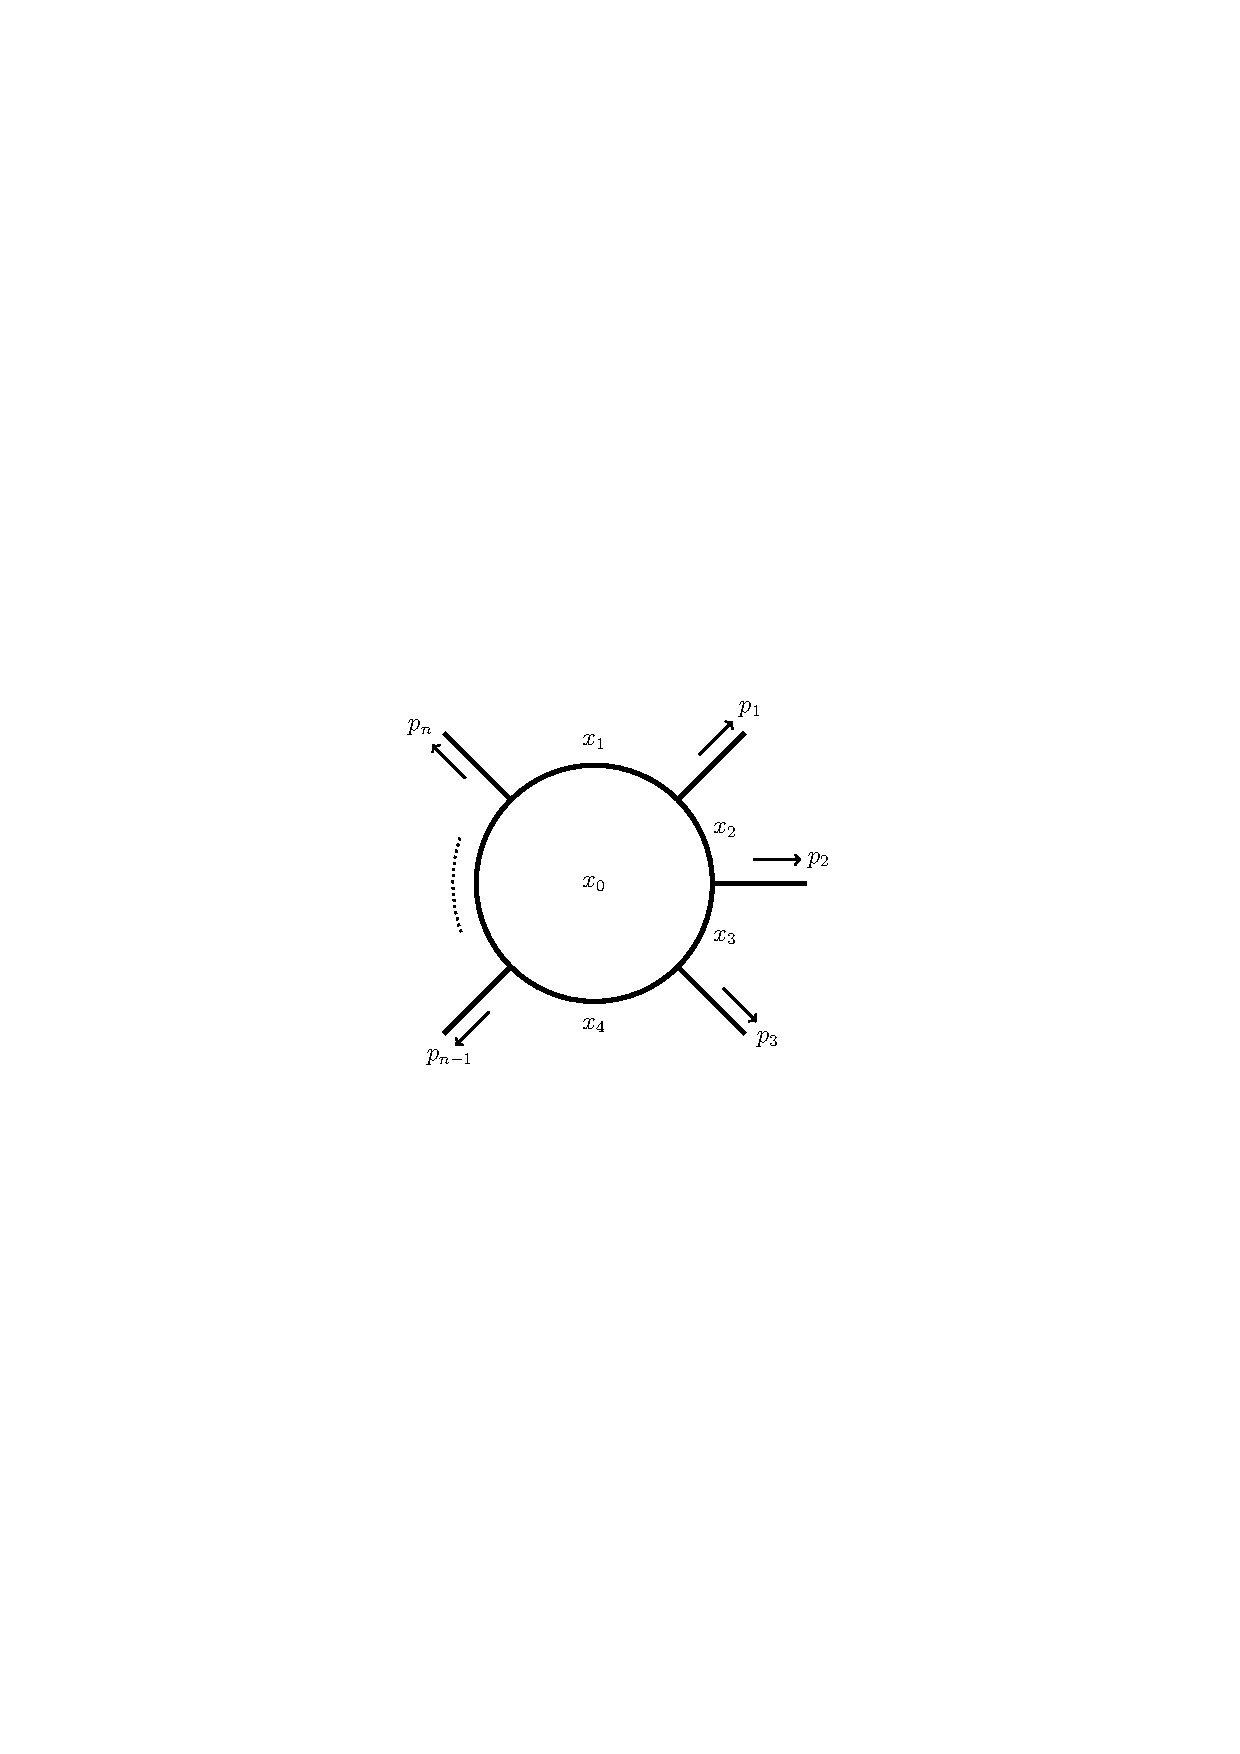
\includegraphics[width=0.5\textwidth]{ch4_loopints/figures/gen1loop-dual.pdf}
   \caption{Generic one-loop $n$-point Feynman diagram and dual coordinates $x$. The latter denote the different dual regions. 
   }
\label{fig:feyn1dualcoordinates}
\end{figure}



Let us consider a generic one-loop scalar $n$-point Feynman integral, as in chapter~\ref{ch:loopamps}, 
%\begin{align}
%\begin{aligned}
%& F^{1-{\rm loop}}_{n} = \int \frac{\d^{D}k}{\i \pi^{D/2}} \times \\
%& \hspace{0.4cm} \times \frac{1}{\bigl[-k^2+m_1^2\bigr]^{a_1} \bigl[- (k+p_1 )^2 + m_2^2\bigr]^{a_2} \ldots \bigl[- (k+p_1 + \ldots + p_{n-1})^2 + m_n^2\bigr]^{a_n} }\,,
%\end{aligned}
%\end{align}
%
\begin{align}
\begin{aligned}
F^{1-{\rm loop}}_{n} = & \int \frac{\d^{D}k}{\i \pi^{D/2}} \frac{1}{\bigl[-k^2+m_1^2\bigr]^{a_1}}  \\
& \times \frac{1}{ \bigl[- (k+p_1 )^2 + m_2^2\bigr]^{a_2} \ldots \bigl[- (k+p_1 + \ldots + p_{n-1})^2 + m_n^2\bigr]^{a_n} }\,,
\end{aligned}
\end{align}
%
see fig.~\ref{fig:onelooppic}, where the external momenta $p_{i}$ may or may not satisfy on-shell conditions.
It is convenient to introduce \emph{dual}, or \emph{region coordinates} $x_i$. 
Each dual coordinate labels one of the regions that the Feynman diagram separates the plane into, as in fig.~\ref{fig:feyn1dualcoordinates}.\footnote{For this purpose, we view the external legs as extending to infinity.} The momentum flowing in each of the edges of the graph is then given by the difference of the coordinates of the adjacent dual regions,
\begin{align} \label{eq:dual_coordinates}
k = x_{1} - x_{0}\,, \quad p_{j} = x_{j+1} - x_{j} \,,
\end{align}
with the identification $x_{j+n} \equiv x_{j}$. 
Then the integral above takes the simple form
\begin{align}\label{oneloop_dual}
F^{1-{\rm loop}}_{n} = \int \frac{\d^{D}x_{0}}{\i \pi^{D/2}} \prod_{j=1}^{n} \frac{1}{ \bigl(- x_{0j}^2 + m_{j}^2 \bigr)^{a_{j} } } \,,
\end{align}
where $x_{ij} \coloneqq x_{i} - x_{j}$.
Translation invariance in the dual space corresponds to the freedom of redefining the loop integration variables $k$ in the initial
integral. Momentum conservation implies that the external momenta form a closed polygon in dual space, with the vertices being the dual coordinates $x_{i}$ and the edges being the momenta $p_{i}$.

 \subsection{Feynman parametrisation}
\label{subsec:Feynmanparam}

It is often convenient to exchange the integration over space-time for parametric integrals. 
Formulae for doing so for general Feynman integrals are given in ref.~\cite{ch4Smirnov:2012gma}. 

The idea of Feynman parametrisation is to exchange the space-time integration for a certain number of auxiliary integrations (over Feynman parameters).
This can be done systematically. 
Let us show how it is done explicitly at one loop. 
The starting point is the general one-loop integral given in \eqn{oneloop_dual}.
The goal is to relate this to the case in \eqn{single_propagator},
by introducing auxiliary integration parameters. 

This method is closely related to the Schwinger formula~\eqref{schwinger} encountered earlier.
The Feynman trick is based on the following identity:
%
\begin{align}\label{Schwinger2}
\frac{1}{X_1^{a_1} X_2^{a_2 }} = \frac{\Gamma(a_1 + a_2 )}{\Gamma(a_1 ) \Gamma(a_2 )}  \int_0^\infty \frac{\d\alpha_1 \d\alpha_2}{{\rm GL}(1)} \frac{ {\alpha_1}^{a_1-1} {\alpha_2}^{a_2-1}}{ (\alpha_1 X_1 + \alpha_2 X_2 )^{a_1 + a_2} } \,.
\end{align}
The RHS of this formula requires some explanation. The form on the RHS is invariant under general linear (GL) transformations, i.e.\ arbitrary rescalings of $\alpha_1$ and $\alpha_2$. The measure ${\d\alpha_1 \d\alpha_2}/{{\rm GL}(1)}$ means that one ``mods out'' by such transformations, so that in effect the integration is only one-dimensional. For example, one could fix $\alpha_2 = 1$, upon which the integration measure becomes $\int_0^\infty \d\alpha_1$. Another common choice is to set $\alpha_1 + \alpha_2 = 1$.  In other words, modding out by the ${\rm GL}(1)$ transformations amounts to inserting a Dirac $\delta$ function---e.g.\ $\delta(\alpha_1+\alpha_2-1)$ or $\delta(\alpha_2-1)$---under the integral sign in \eqn{Schwinger2}.

Feynman integrals typically have many propagators (corresponding to the number of edges), so we need 
a generalisation of \eqn{Schwinger2} to an arbitrary number $n$ of denominator factors:
\begin{align}\label{Feynman_general}
\frac{1}{ \prod_{i=1}^{n}  X_i^{a_i} }  = \frac{\Gamma(a_1 + \ldots + a_n) }{\prod_{i=1}^{n} \Gamma(a_i )}  \int_0^\infty \frac{ \prod_{i=1}^{n}  \d\alpha_i  }{{\rm GL}(1)}    
\frac{  \prod_{i=1}^{n}    \alpha_i^{a_i-1}  } { (\sum_{i=1}^{n} \alpha_i X_i)^{a_1 + \ldots + a_n } }\,.
\end{align}
This can be shown by mathematical induction.


Applying \eqn{Feynman_general} to the one-loop formula~\eqref{oneloop_dual} yields an integral over a single factor in the integrand.
By performing a change of variables in the integration variables $k$, this can be brought into the form of \eqn{single_propagator},
and hence the space-time integration can be performed (see exercise~\ref{Ex:MasslessBubble} for an example).
The result is
%
\begin{align}\label{oneloop_master}
F_{n} =  
\frac{\Gamma(a-D/2)}{\prod_{i=1}^{n} \Gamma(a_{i})}  
\int_{0}^{\infty}  \frac{   \prod_{i=1}^{n} 
 \d\alpha_{i} \alpha_{i}^{a_{i}-1} }{ {\rm GL}(1)} 
\frac{U^{a-D} }{ (V + U \sum_{i=1}^{n} m_{i}^2 \alpha_i  -\i 0)^{a-D/2}} \,,
\end{align}
where $U = \sum_{i=1}^{n} \alpha_{i}$ and $V = \sum_{i<j} \alpha_i \alpha_j (-x_{ij}^2)$.
These polynomials, called \emph{Symanzik polynomials}, have a graph-theoretical interpretation, see e.g.~\cite{ch4Smirnov:2012gma}. 
Consider the graph corresponding to the propagators forming the loop, where an edge corresponding to a denominator $X_i$ has label $\alpha_i$. 
Then, consider all ways of removing a minimal number of lines so that the graph becomes a tree. To each such term, associate the product of $\alpha_i$ factors of the removed factors. Summing over all such terms gives $U$. Similarly, to define $V$, one considers all ways of removing factors to obtain two trees, and again takes the products of the $\alpha_i$, but this time weighted by (minus) the momentum squared flowing through these lines, which yields $-\alpha_i \alpha_j x_{ij}^2$ at one loop.

Depending on the situation, different choices of fixing the  ${\rm GL}(1)$ invariance in \eqn{oneloop_master} may be particularly convenient. One may fix $U=1$, for example, or alternatively one may set one of the Feynman parameters $\alpha_i$ to $1$.


\begin{figure}[h]
  \begin{subfigure}{0.5\textwidth}
    \centering
    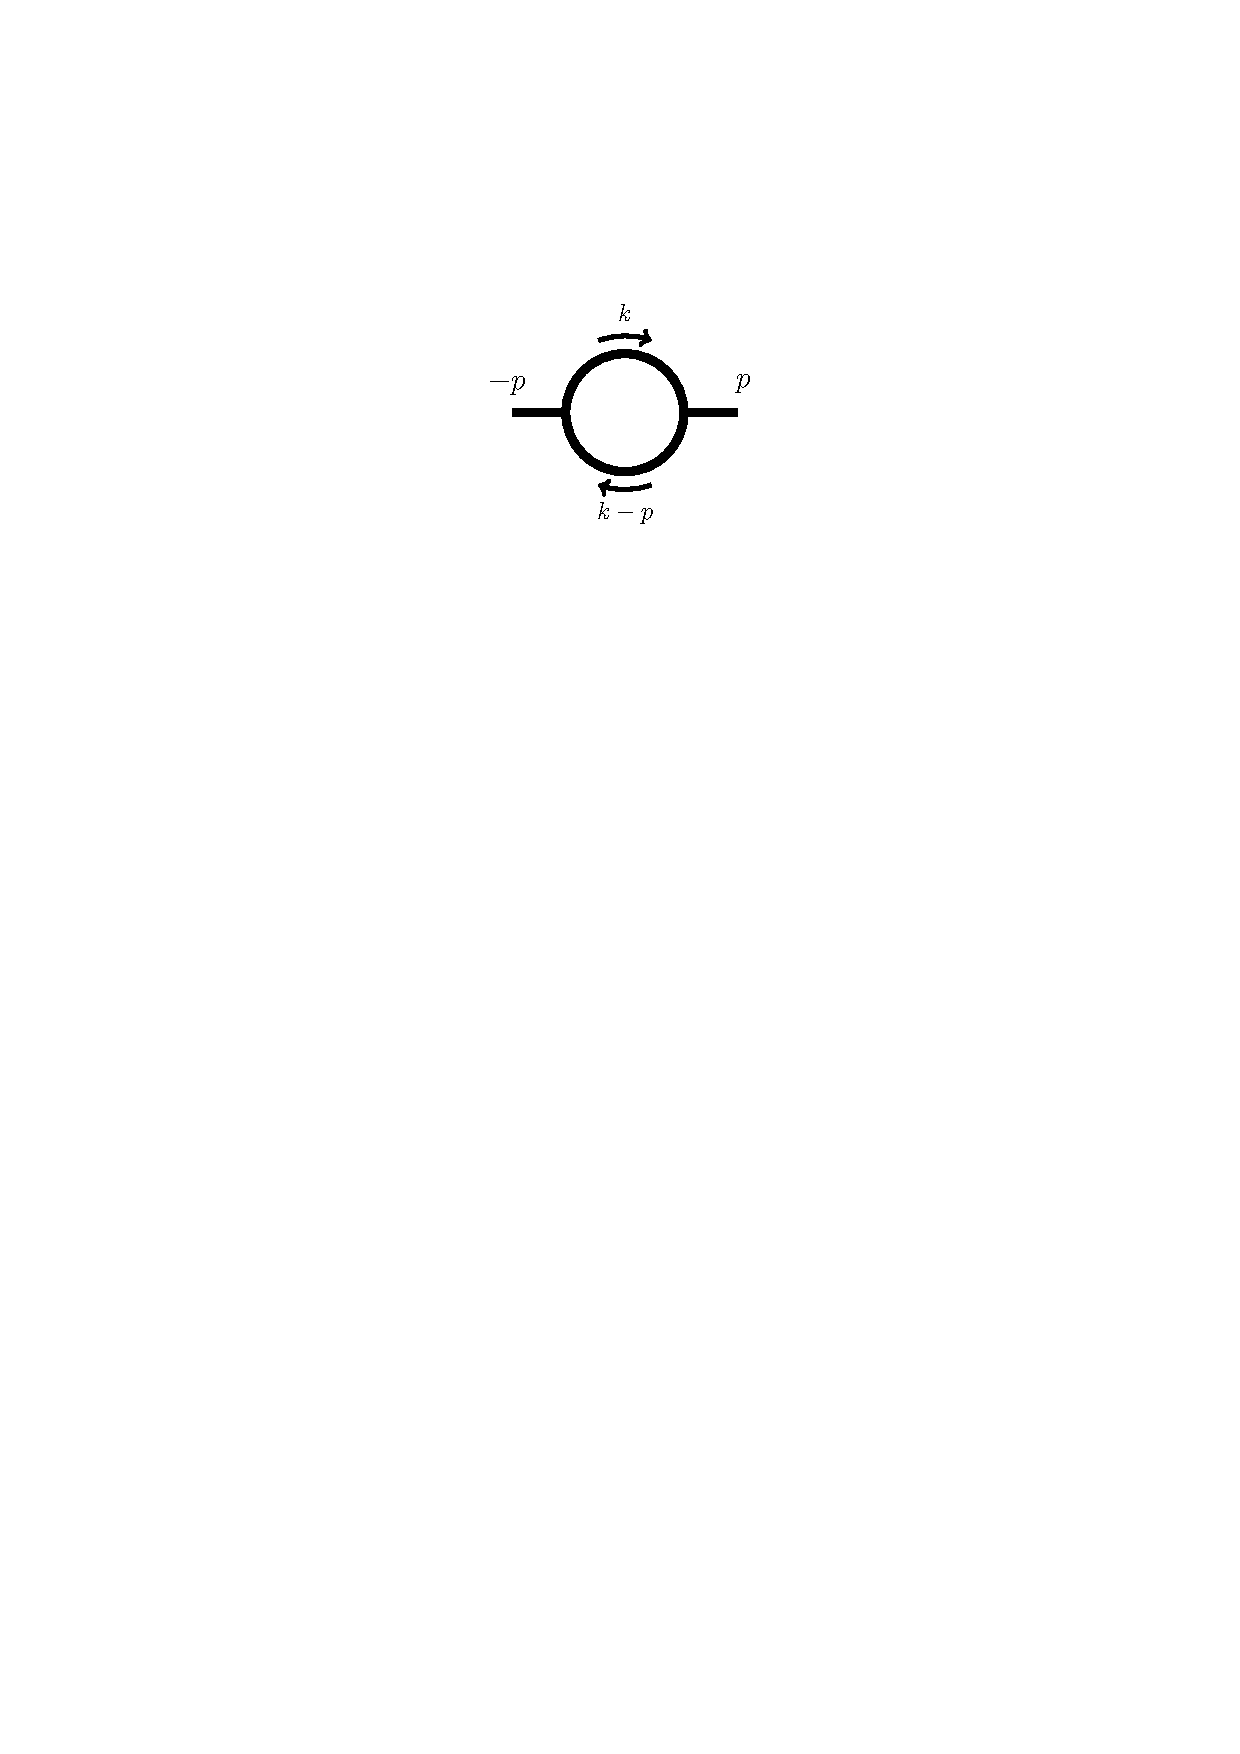
\includegraphics[width=0.7\textwidth]{ch4_loopints/figures/bubblewithlabels.pdf}
     \caption{}
    \label{fig:feynbubbleandtriangle-bubble}
    \quad\quad\quad\quad\quad\quad
  \end{subfigure}
  %
  \begin{subfigure}{0.4\textwidth}
    \centering
    \vspace*{-4mm}
    \hspace*{-6mm}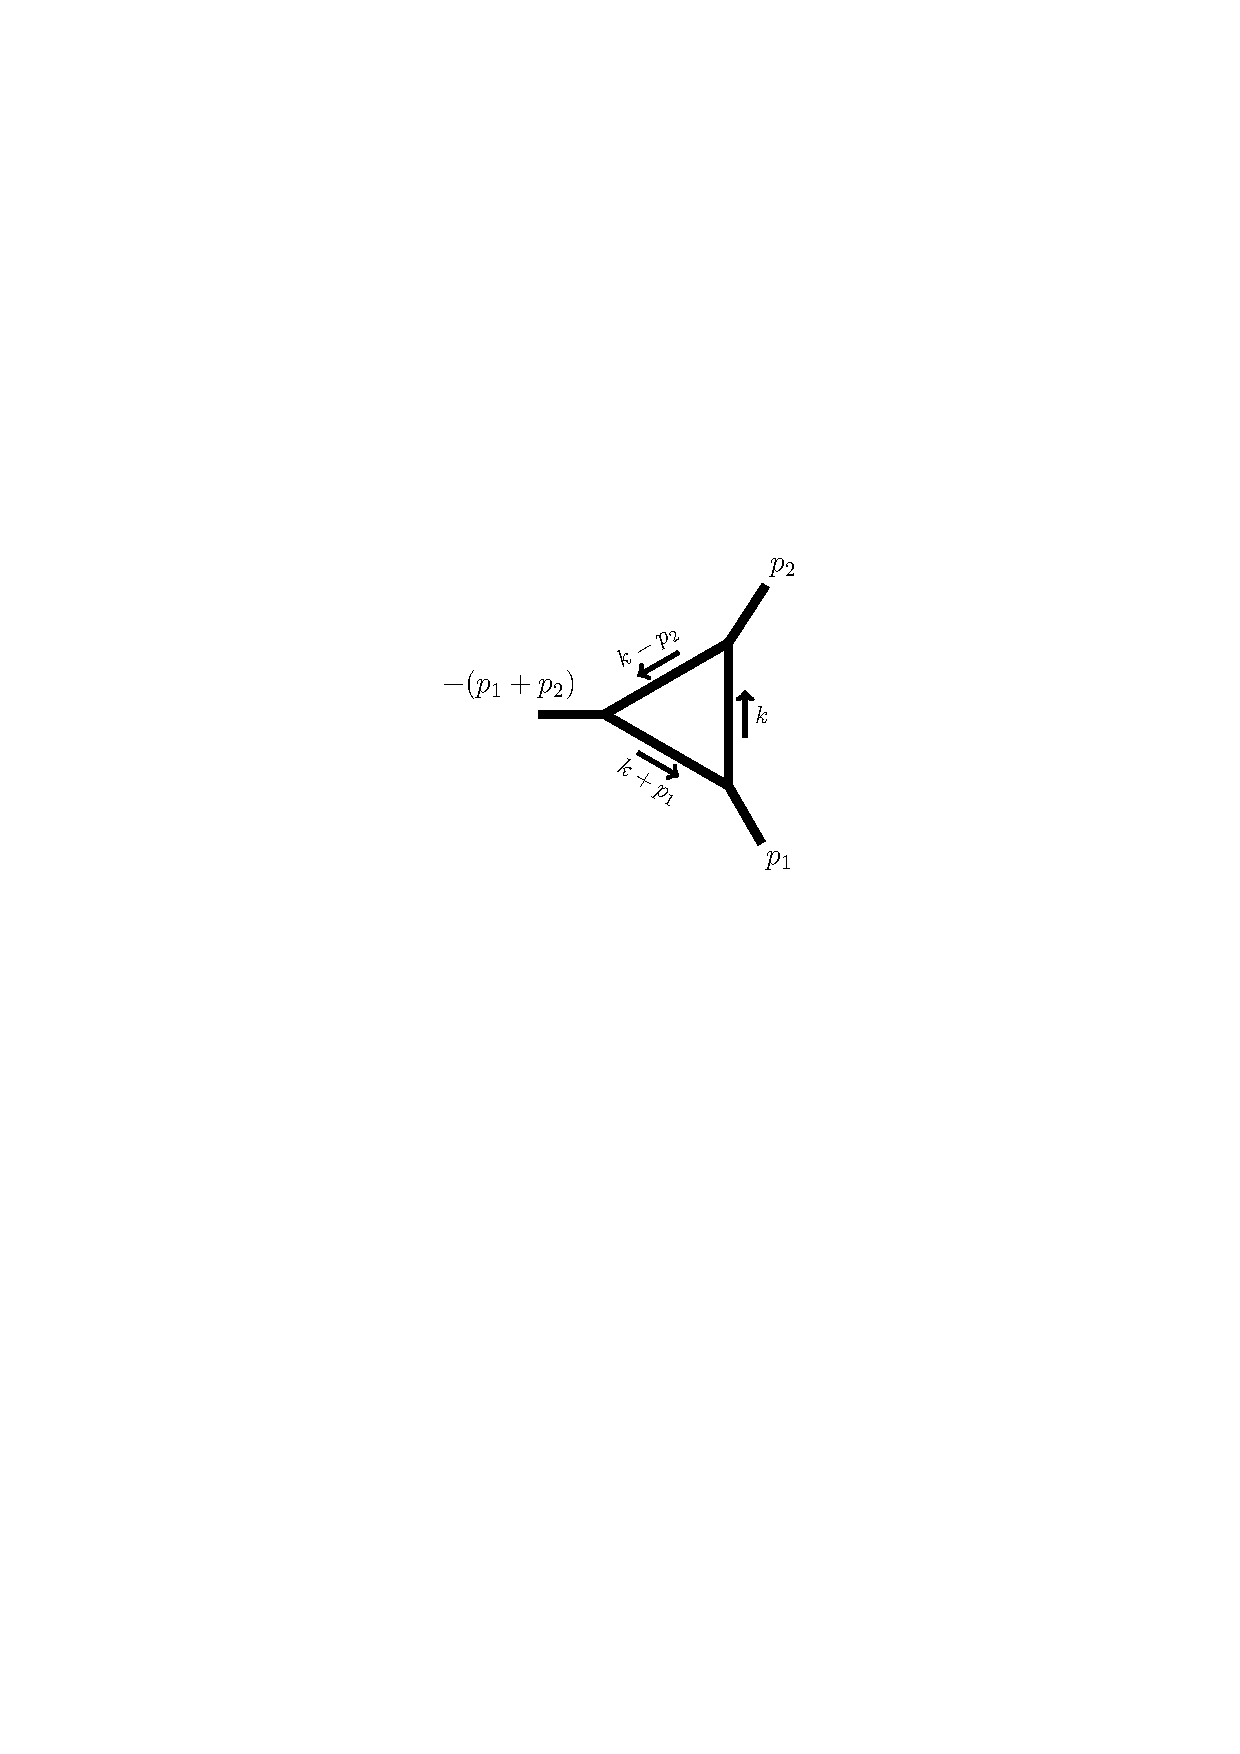
\includegraphics[width=0.85\textwidth]{ch4_loopints/figures/trianglewithlabels.pdf}
    \caption{}
    \label{fig:feynbubbleandtriangle-triangle}
  \end{subfigure}
  \caption{Bubble and triangle Feynman integrals discussed in the main text. The arrows denote the direction of the momenta.}
  \label{fig:feynbubbleandtriangle}
\end{figure}


\newpage

\begin{exer}{The massless bubble integral}
\label{Ex:MasslessBubble}
%
Consider the bubble integral, cf. fig.~\ref{fig:feynbubbleandtriangle-bubble}, with massless propagators but generic propagator powers:
\begin{align} \label{eq:massless_bubble}
F_{2}\left( a_1,a_2 ; D\right) = \int \frac{\d^D k}{\i \pi^{\frac{D}{2}}} \frac{1}{\left(-k^2  - \i 0\right)^{a_1} \left(-(k-p)^2  - \i 0 \right)^{a_2} } \,.
\end{align}

\begin{enumerate}[a)]

\item Use the identity~\eqref{Schwinger2} to write down the Feynman parameterisation. Verify that it matches the general formula~\eqref{oneloop_master}, and read off the Symanzik polynomials.

\smallskip
\item Show that the integral evaluates to
\begin{align} \label{eq:Ibubblechapter4}
F_{2}\left( a_1,a_2 ; D \right) = B\left(a_1, a_2 \right) \, \bigl(-p^2 - \i 0 \bigr)^{\frac{D}{2}-a_1-a_2} \,,
\end{align}
with
\begin{align} \label{eq:Bbubble}
B\left(a_1,a_2 ; D\right) = \frac{\Gamma\left(a_1+a_2-\frac{D}{2}\right) \Gamma\left(\frac{D}{2}-a_1\right) \Gamma\left(\frac{D}{2}-a_2\right)}{\Gamma\left(a_1\right) \Gamma\left(a_2\right) \Gamma\left(D-a_1-a_2\right)} \,.
\end{align}

\end{enumerate}
%
For the solution see \hyperref[Sol:MasslessBubble]{chapter~5}.
\end{exer}



\begin{example}{Example: Infrared-divergent massless triangle integral}

As an example of the one-loop Feynman parameter formula~\eqref{oneloop_master}, let us consider the massless on-shell triangle diagram of fig.~ \ref{fig:feynbubbleandtriangle-triangle},
\begin{align}\label{F3examplemomentumspace}
F_3 =  \int \frac{\d^{D}k}{\i \pi^{D/2}} \frac{1}{[-k^2 -\i 0] [-(k+p_{1})^2-\i 0] [- (k-p_{2})^2 -\i 0]} \,.
\end{align}
In order to use \eqn{oneloop_master}, we need to match the kinematics to the general notation used there.
Note that \eqn{F3examplemomentumspace} is a special case of \eqn{oneloop_dual} with $n=3$ and the following choices:
zero particle masses $m_1=m_2=m_3=0$, and unit propagator exponents $a_1 = a_2= a_3 =1$.
Moreover, we consider the massless on-shell conditions $p_{1}^2= p_{2}^2 = 0$, 
so that the integral depends on the dimensionful variable $s = (p_{1}+p_{2})^2$, and on $D$.
Translating this to dual coordinates, we have $x_{12}^2= 0, x_{23}^2=0, x_{13}^2 =s$.
\begin{exer}{Feynman parametrisation}
\label{Ex:4.FeynPar}
Draw the triangle diagram in \eqn{F3examplemomentumspace} using both the momentum-space and the dual-space labelling, and verify the above identification of variables.
Use this to write down the Feynman parametrisation for $F_{3}$.
For the solution see \hyperref[Sol:4.FeynPar]{chapter~5}.
\end{exer}

%
Having established this notation, we can readily employ our main one-loop formula~\ref{oneloop_master}.
Setting $D=4-2 \eps$, it gives
\begin{align}\label{F3triangleFeynman}
F_3 =  \int_0^{\infty} \frac{ \d\alpha_1 \d\alpha_2 \d\alpha_3}{{\rm GL}(1)} \frac{\Gamma(1+\eps)}{(-s \, \alpha_1 \alpha_3 -\i 0)^{1+\eps} (\alpha_1 + \alpha_2 + \alpha_3 )^{1-2\eps} } \, .
\end{align}
For simplicity, let us consider the so-called Euclidean kinematic region, where $s<0$. In this case, we see that the denominator on the RHS is positive, and therefore the $\i 0$ prescription is not needed. 
Later we may be interested in analytically continuing the integral to other kinematic regions. Noticing that the $\alpha$-parameter polynomial multiplying $-s$ is positive, we can conveniently record the information on the correct analytic continuation prescription  by giving a small imaginary part to $s$: $s \to s + \i 0$.
In the present case, the dependence on $s$ is actually trivial: it is dictated by the overall dimensionality of the integral.
This implies that $F_3$ depends on $s$ as $(-s-\i 0)^{-1-\eps}$.

Let us comment on the convergence properties of \eqn{F3triangleFeynman}.
The expression is valid for $\eps<0$. 
This is consistent with our expectations, since this integral is UV-finite (see the power counting in \eqn{eq:UVpowercounting}) but has IR divergences.
The integral would actually be finite for $p_1^2 \neq 0, p_2^2 \neq 0$.
For on-shell kinematics $p_1^2=p_2^2=0$, one can see there are problematic regions of loop momentum in \eqn{F3examplemomentumspace}
that lead to divergences when integrating in $D=4$ dimensions. 
The soft region occurs when all components of $k$ in \eqn{F3examplemomentumspace} are small. 
On top of this, there are two collinear regions, where $k \sim p_1$ and $k\sim p_2$, respectively. 
One may convince oneself by power counting (see e.g.~\cite{ch4Agarwal:2021ais}  
for more details) that these regions lead to logarithmic divergences ($1/\eps$ in dimensional regularisation).
Moreover, each collinear region overlaps with the soft region, so that the divergences can appear simultaneously. 
We therefore expect the leading term of $F_3$ as $\eps \to 0$ to be a double pole $1/\eps^2$.


Let us now verify this explicitly.
In order to carry out the $\alpha$ integrals we introduce the following useful formula,
\begin{align}\label{alpha_integrals}
\int_0^\infty \frac{\prod_{i=1}^{n} \d\alpha_{i}\,
\alpha_{i}^{b_i-1}}{{\rm GL}(1)} \biggl(\sum_{i=1}^{n} \alpha_i \biggr)^{-b} = \frac{ \prod_{i=1}^{n} \Gamma(b_i )} {\Gamma( b)} \,,\quad {\rm with} \quad b=\sum_{i=1}^{n} b_i\,.
\end{align}
Applying this to \eqn{F3triangleFeynman}, for $b_1=-\eps, b_2 = 1, b_3=-\eps$,  we find
\begin{align}
F_{3} = (-s-\i 0)^{-1-\eps} \frac{\Gamma(1+\eps) \Gamma^2(-\eps)}{\Gamma(1-2 \eps)} \,.
\end{align}
We wish to expand this formula for small $\eps$. To do so, we need to familiarise us with the properties of the $\Gamma$ function.

\begin{svgraybox}
{\bf Important properties of the $\Gamma$ function.}
In the calculation above we encountered a first special function, the $\Gamma$ function.
It is defined as 
\begin{align}
\Gamma(x) = \int_0^\infty \d t \, t^{x-1} \mathrm{e}^{-t} \,.
\end{align}
This formula converges for $x >0$. To define $\Gamma(x)$ for complex $x$, one uses analytic continuation.
Here we collect several important properties of the $\Gamma$ function.
%
It satisfies the recurrence
\begin{align} \label{eq:gammarecurrence}
\Gamma(x+1) = x \, \Gamma(x) \,.
\end{align}
It has the expansion
\begin{align} \label{eq:logGammaTaylor}
\log \Gamma(1+x) = - \gamma_{\text{E}} \, x + \sum_{n=2}^{\infty} \frac{(-1)^n \, x^n}{n} \zeta_n \,,
\end{align}
for $|x|<1$.
Here, Euler's constant is
\begin{align} \label{eq:EulerConstant}
\gamma_{\text{E}} = - \Gamma'(1) = 0.57721\ldots \,,
\end{align}
and Riemann's zeta constants appear,
\begin{align} \label{eq:zetan}
\zeta_n = \sum_{k=1}^{\infty} \frac{1}{k^n}  \,, \qquad \forall \, n\ge 2 \,.
\end{align}
For even $n$, these evaluate to powers of $\pi$, e.g.\ 
$\zeta_2 = \pi^2/6$ and $\zeta_{4} = \pi^4/90$.
\end{svgraybox}
Using the expansion~\eqref{eq:logGammaTaylor}, as well as \eqn{eq:gammarecurrence}, we find
\begin{align}
\mathrm{e}^{\eps \gamma_{\rm E}} F_{3} =  (-s)^{-1-\eps} \left[ \frac{1}{\eps^2} - \frac{\pi^2}{12} - \frac{7}{3} \zeta_3 \eps - \frac{47 \pi^4}{1440} \eps^2 + \cO(\eps^3)\right]\,.
\end{align}
Here we multiplied $F_{3}$ by a factor of $\mathrm{e}^{\eps \gamma_{\rm E}}$ (in general, one takes one
such factor per loop order),
in order to avoid the explicit appearance of $\gamma_{\rm E}$ in the expansion.
\end{example}


\begin{exer}{Taylor series of the Log-Gamma function}
\label{Ex:TaylorLogGamma}
%
In this guided exercise we prove the Taylor series of the Log-Gamma function in \eqn{eq:logGammaTaylor}. 
The Taylor series of $\log \Gamma(1+x)$ around $x=0$ is given by
\begin{align} \label{eq:loggammataylorgen}
\log \Gamma(1+x) = \sum_{n=1}^{\infty} \frac{x^n}{n!} \left( \frac{\d^n}{\d x^n} \log \Gamma(1+x) \right)\biggl|_{x=0} \,.
\end{align}
The first-order derivative by definition gives Euler's constant $\euler$~\eqref{eq:EulerConstant}.
In order to compute the higher-order derivatives, we derive a series representation for the \emph{digamma function} $\psi(x)$, i.e.\ the logarithmic derivative of the gamma function,
\begin{align} \label{eq:psidef}
\psi(x) \coloneqq \frac{\d \log \Gamma(x)}{\d x} = \frac{\Gamma'(x)}{\Gamma(x)} \,.
\end{align}

\begin{enumerate}[a)]

\item Prove the following recurrence relation for the digamma function,
\begin{align} \label{eq:psixn}
\psi(x+n) = \psi(x) + \sum_{k=0}^{n-1} \frac{1}{x+k} \,, \qquad n \in \mathbb{N}\,.
\end{align}

\item Prove the following series representation of the digamma function,
\begin{align} \label{eq:psiseries}
\psi(x) = - \gamma_{\text{E}} - \sum_{k=0}^{\infty} \left(\frac{1}{x+k}-\frac{1}{1+k} \right) \,.
\end{align}
Hint: study the limit of $\psi(x+n)-\psi(1+n)$ for $n\to \infty$ using Stirling's formula,
\begin{align} \label{eq:stirling}
\Gamma(x+1) = \sqrt{2 \pi x} \, x^x \, \text{e}^{-x} \left[1 + \mathcal{O}\bigl(1/x\bigr) \right] \,.
\end{align}

\item Use \eqn{eq:psiseries} to prove the Taylor series in \eqn{eq:logGammaTaylor}.

\end{enumerate}
For the solution see \hyperref[Sol:TaylorLogGamma]{chapter~5}.
\end{exer}





\begin{example}{Example: Ultraviolet divergent bubble integral}

An important example throughout this chapter will be the one-loop massive bubble integral.
The integral is defined as
\begin{align}
F_{2}(s,m^2;D) = \int \frac{\d^{D}k}{\i \pi^{D/2}} \frac{1}{(-k^2+m^2 - \i 0) [-(k-p)^2+m^2- \i 0]} \,.
\label{defbubble}
\end{align}
The integrated function depends on the external momentum $p$ via the Lorentz invariant $s=p^2$.
This is a special case of \eqn{oneloop_dual} with $n=2$, with uniform internal masses $m_1=m_2=m$, with unit propagator powers $a_1=a_2=1$, and with the single kinematic variable $x_{12}^2=p^2$.
In slight abuse of notation, we denote this integral by the same letter $F_2$ as we did for the massless bubble integral above.

Applying \eqn{oneloop_master}, we find
\begin{align}\label{eq:bubbleFeynman} 
F_{2}(s,m^2;D) = \Gamma\left(2-\frac{D}{2}\right)  \, \int_0^\infty \frac{\d \alpha_1 \d\alpha_2}{{\rm GL}(1)} 
\frac{(\alpha_1+\alpha_2)^{2-D} }{[\alpha_1 \alpha_2 (-s) + (\alpha_1 + \alpha_2)^2 m^2 -\i 0]^{2-D/2}  } \,.
\end{align} 
Just as in the triangle example above, we see that the integrand in this formula is positive definite in the Euclidean region $s<0, m>0$, and that we can absorb the $\i 0$ prescription into $s$.

We see that $\Gamma(2-D/2)$ is divergent for $D \to 4$, and requires $D<4$ for convergence. The parameter integral is instead well-defined for $D=4$. Therefore we can compute the integral for $D=4-2\eps$, with $\eps>0$. In the limit $\eps\to0$, we find
\begin{align}\label{BleadingpoleUV}
 F_{2}(s,m^2;D) = 
 \frac{1}{\eps}  
 + 
 {\mathcal{O}}\bigl(\eps^0\bigr)
  \,.
\end{align}
This divergence is of ultraviolet origin. As we discussed in chapter~\ref{ch:loopamps}, we can understand it by doing power counting in the momentum-space representation~\eqref{defbubble}. Consider the integrand for large loop momentum $k$. Switching to radial coordinates, the integration measure becomes $\d^{D}k = r^{D-2} \d r \, \d\Omega$, where $r$ is the radial direction, and $\Omega$ represents the angular integrations. At large $r$, the integrand goes as $\d r/r^{D-4}$. This converges for $D<4$, but leads to a logarithmic divergence at $D=4$. This is exactly what \eqn{BleadingpoleUV} encodes.
With the same power counting, we see that the integral in \eqn{defbubble} is finite in $D=2$. 
\end{example}

\begin{exer}{Finite two-dimensional bubble integral}
\label{Ex:4.2Dbubble}
Starting from the Feynman parametrisation in eq. (\ref{eq:bubbleFeynman}), carry out the remaining integration for $D=2$, for the kinematic region $s<0, m^2>0$, to find
\begin{align}\label{resbubbleexplicit}
F_{2}\bigl(s,m^2;D=2\bigr) =  \frac{2}{s \, \sqrt{1-4 m^2/s}} \log \left(  \frac{\sqrt{1-4 m^2/s}-1}{\sqrt{1-4 m^2/s}+1} \right) \,.
\end{align}
Hint: employ the change of variables $-s/m^2 = (1-x)^2/x$, with $0<x<1$.
For the solution see \hyperref[Sol:4.2Dbubble]{chapter~5}.
\end{exer}
We will also be interested in the dimensionally-regularised version of \eqn{defbubble}, i.e.\ the deformation where $D=2-2 \epsilon$. 
This is interesting for several reasons. Firstly, we have seen in chapter~3 that integrals in dimensions $D$ and $D\pm 2$ are related by certain recurrence relations, see \eqn{eq:dimshift} at one-loop order~\cite{ch4Lee:2012cn}.
Secondly, this integral for $D=2-2\eps$ will serve as a main example for understanding integration techniques in this chapter.  


Before closing this section, let us mention the $L$-loop generalisation of \eqn{oneloop_master}.
\begin{svgraybox}
{\bf Feynman parametrisation for a scalar $L$-loop Feynman diagram.}
Consider now an $L$-loop scalar Feynman integral with $n$ denominator factors.
The graph may be planar or non-planar. As before, we label the $i$-th factor (which may have a generic mass $m_i^2$ and is raised to a power $a_i$) by the Feynman parameter $\alpha_i$.
Then, the generalisation of \eqn{oneloop_master} is given by
\begin{align}\label{FeynmanLloopgeneralization}
\frac{\Gamma(a-L D/2)}{\prod_{i=1}^{n} \Gamma(a_{i})}  
\int_{0}^{\infty}  \frac{   \prod_{i=1}^{n} 
 \d\alpha_{i} \, \alpha_{i}^{a_{i}-1} }{ {\rm GL}(1)} 
\frac{U^{a-L D} }{ (V + U \sum_{i=1}^{n} m_{i}^2 \alpha_i  -\i 0)^{a-L D/2}} \,.
\end{align}
Here $a= \sum_i a_i$, and the Symanzik polynomials $U$ and $V$ have the same graph theoretical definition mentioned above.
They have been implemented in various useful computer programs, for example~\cite{ch4Lee:2012cn}. 
\end{svgraybox}


\subsection{Summary}
In this section, we introduced conventions and notations for Feynman integrals.
The integrals are initially defined as space-time integrals, but other representations are also useful.
We showed how Feynman  
representations are obtained.
We discussed a number of sample one-loop integrals, and showed how ultraviolet and infrared divergences
are treated in dimensional regularisation. 
We also saw first examples of special functions appearing in the integrated answers, namely the $\Gamma$ function and the logarithm.
In the next sections, we introduce the Mellin-Barnes method, which will allow us to go beyond the cases treated so far, and see first examples of polylogarithms.
After that we discuss more systematically special functions appearing in Feynman integrals,
and propose a useful way for thinking about them in terms of their defining differential equations.



\section{Mellin-Barnes techniques}
\label{section:mellin}

In the previous section we saw how to derive parameter-integral formulae for Feynman integrals.
For a triangle diagram we derived the complete analytic answer by carrying out the parameter integrals,
and we did the same for the finite two-dimensional massive bubble integral.
In general, it is difficult to carry out the Feynman parameter integrals directly (see however interesting work in this direction, together with powerful algorithms~\cite{ch4Panzer:2014caa}).

Another useful representation 
trades the Feynman parameter integrals
for Mellin-Barnes integrals, as we describe 
presently. 
The resulting Mellin-Barnes representations makes certain properties of the integrals easier to see as compared to the Feynman parameter integrals. In particular, useful algorithms have been developed to resolve singularities in $\eps$ and to provide representations of the terms in the Laurent expansion of the Feynman integrals.
%
\begin{figure}[t]
\centering
\begin{tikzpicture}[baseline={(current bounding box.center)}]

  % define value of "a" for \Gamma(z+a)
  \newcommand \aval {1.2};
   
  % draw shaded gray area
  \fill[gray!45] (-\aval,-1.7) rectangle (0,1.7);
    
  % draw axes
  \draw [->] (-4,0) -- (4,0) node [below left, xshift=0.3cm, yshift=-0.05cm]  {$\text{Re}(z)$};
  \draw [->] (0,-1.7) -- (0,1.7) node [below right, xshift=0.05cm] {$\text{Im}(z)$};
  
  % draw ticks
  \foreach \n in {-3,-2,-1,0,1,2,3}{ 
    \draw (\n,-2pt) -- (\n,2pt); % node [above] {$\n$}; 
  }
    
    % vertical dashed line
    \draw[dashed,->] (-\aval/2+0.1, -1.7) -- (-\aval/2+0.1, 1.7);
  
  % poles of \Gamma(-z)
  \draw[mark=x, mark size=4pt] plot (0,0) node[below, xshift=-0.2cm, yshift=-0.1cm] {$0$};
  \draw[mark=x, mark size=4pt] plot (1,0) node[below, yshift=-0.1cm] {$1$};
  \draw[mark=x, mark size=4pt] plot (2,0) node[below, yshift=-0.1cm] {$2$};
  \draw[mark=x, mark size=4pt] plot (3,0) node[below, yshift=-0.1cm] {$3$};

  % poles of \Gamma(a+z)
   \draw[mark=x, mark size=4pt] plot (-\aval,0) node[below, yshift=-0.175cm] {$-a$};
   \draw[mark=x, mark size=4pt] plot (-1-\aval,0) node[below, yshift=-0.1cm] {$-1-a \, \,$};
   \draw[mark=x, mark size=4pt] plot (-2-\aval,0) node[below, yshift=-0.1cm] {$-2-a \, \,$};

\end{tikzpicture}
\caption{Integration contour for Mellin-Barnes representation in eq.~(\ref{MB_basic}). The integration contour (dashed line) goes parallel to the vertical axis, with ${\rm Re}(z)=c$, with $-a<c<0$, i.e.\ to the right of the poles of $\Gamma(-z)$, and to the left of the poles of  $\Gamma(z+a)$ (shaded~area).}
\label{fig:mb1}
\end{figure}
%
The key formula is the following,
\begin{align}\label{MB_basic}
\frac{1}{(x+y)^{a}} = \frac{1}{\Gamma(a)} \, \int_{c - \i \infty}^{c+\i \infty} \frac{\d z}{2 \pi \i} \, \Gamma(-z) \Gamma(z+a) \, x^z y^{-a-z} \,,
\end{align}
where the integration contour is parallel to the imaginary axis, with real part $c$ in the interval $-a<c<0$.
See Fig.~\ref{fig:mb1}. In general, the integration contour is chosen such that the poles of $\Gamma$ functions of the type $\Gamma(z+\ldots )$ lie to its left, and the poles of  $\Gamma(-z+\ldots)$ lie to its right.

One can verify the validity of \eqn{MB_basic} by checking that the series expansions of its LHS and RHS agree.
Let us see this in detail.
Assume $x<y$. Then the LHS of \eqn{MB_basic} has the following series representation,
\begin{align}\label{MB_check}
\frac{1}{(x+y)^{a}} = y^{-a} \sum_{n\ge 0} \, (-1)^{n+1} \frac{ \Gamma(n+a)}{\Gamma(n+1)\Gamma(a)} \left( \frac{x}{y} \right)^n \,,\qquad x<y\,.
\end{align}
Let us see how this arises from the RHS of \eqn{MB_basic}. If $x<y$ we can close the integration contour in \eqn{MB_basic} on the right,
because the contribution from the semicircle at infinity vanishes.
By complex analysis, we get a contribution from (minus) all poles of $\Gamma(-z)$ situated at $z_{n} = n$, with $n = 0, 1, \ldots$.
Taking into account that the corresponding residues are $\text{Res}[\Gamma(-z), \, z=n]=(-1)^{n+1}/n!$ (see exercise~\ref{Ex:ExpGamma}),
one readily reproduces \eqn{MB_check}.
One may verify similarly the validity of \eqn{MB_basic} for $y<x$. In this case, one closes the integration contour on the left.

Equation~\eqref{MB_basic} can be used to factorise expressions, e.g.\ the denominator factors appearing 
in Feynman parametrisation.
Once factorised, \eqn{alpha_integrals} 
allows one to carry out the Feynman parameter integrals. 
In some sense, the Mellin-Barnes representation can therefore be considered
the inverse of the Feynman parametrisation.
Of course, this means that one is just trading one kind of integral representation for another.
However, the Mellin-Barnes representation is very flexible, and has a number of useful features, as
we will see shortly.



\begin{exer}{Laurent expansion of the Gamma function}
\label{Ex:ExpGamma}
%
The Gamma function $\Gamma(z)$ is holomorphic in the whole complex plane except for the non-positive integers, $z=0,-1,-2,\ldots$, where it has simple poles. 

\begin{enumerate}[a)]
\item Compute the Laurent expansion of $\Gamma(z)$ around $z=0$ up to order $z$,
\begin{align} \label{eq:GammaExp0}
\Gamma(z) = \frac{1}{z} - \gamma_{\text{E}} + \frac{z}{2}\left(\euler^2 + \zeta_2\right) + \mathcal{O}\left(z^2 \right)\,.
\end{align}

\item Using eq.~\eqref{eq:GammaExp0}, show that the Laurent expansion of $\Gamma(z)$ around $z=-n$, with $n\in\mathbb{N}_0$, is given by
\begin{align} \label{eq:GammaExpn}
\Gamma(z) = \frac{(-1)^n}{n!} \left\{ \frac{1}{z+n} + H_n-\euler + \frac{1}{2}(z+n) \left[\left(H_n - \euler\right)^2 + \zeta_2 + H_{n,2} \right] \right\} + \ldots \,,
\end{align}
where the ellipsis denotes terms of order $(z+n)^2$ or higher. Here, $H_{n,r}$ is the $n$-th harmonic number of order $r$,
\begin{align}  \label{eq:harmonicnumbers}
H_{n,r} \coloneqq \sum_{k=1}^n \frac{1}{k^r} \,, \qquad \qquad H_{n} \coloneqq H_{n,1} \,.
\end{align}

\end{enumerate}
For the solution see \hyperref[Sol:ExpGamma]{chapter~5}.
\end{exer}




\subsection{Mellin-Barnes representation of the one-loop box integral}

\begin{figure}[t]
  \centering
  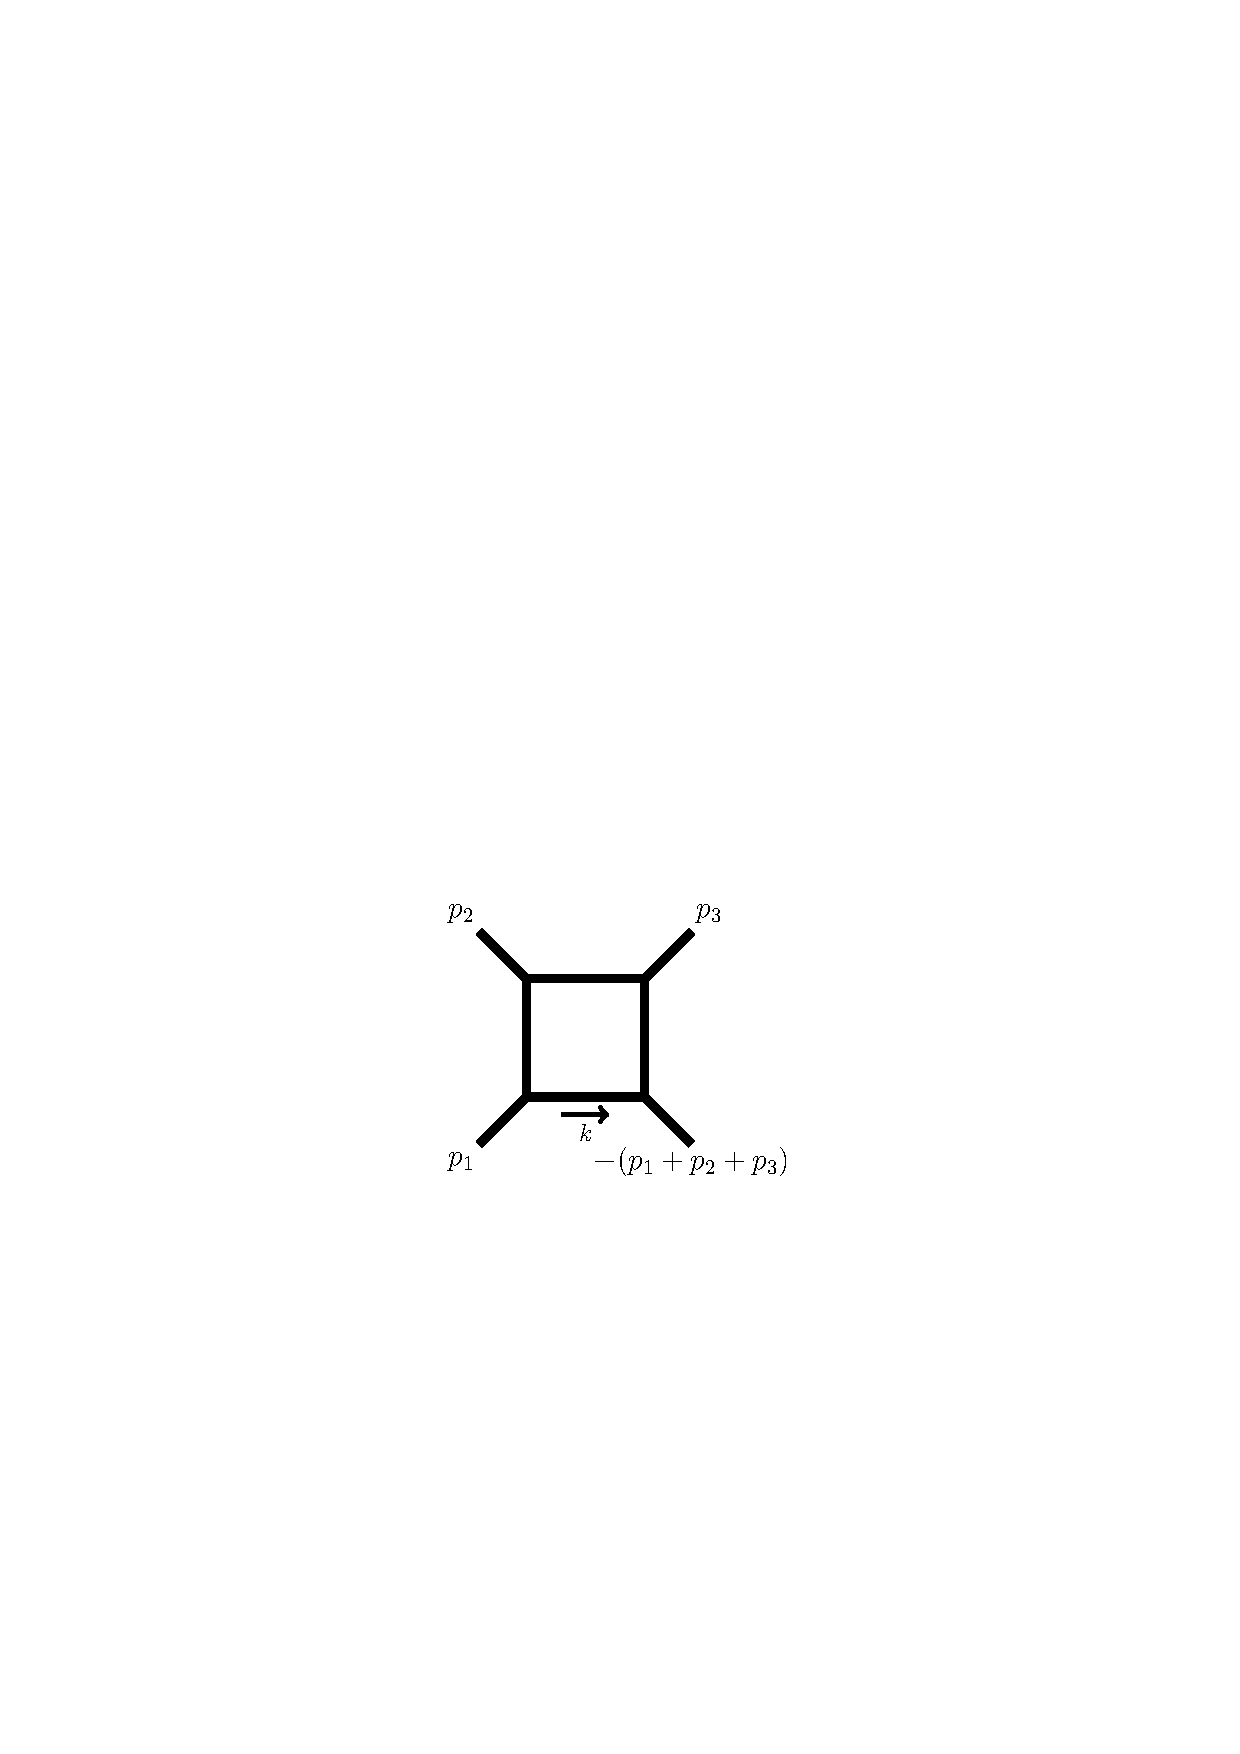
\includegraphics[width=0.4\textwidth]{ch4_loopints/figures/boxwithlabels.pdf}
  \caption{Massless one-loop four-point Feynman integral considered in the main text.}
  \label{fig:mb2}
\end{figure}

Let us apply the above procedure to the massless one-loop box integral,
cf.~fig.~\ref{fig:mb2}:
\begin{align}
F_{4} = \int \frac{\d^{D}k}{\i \pi^{D/2}} \frac{1}{k^2 (k+p_1)^2 (k+p_1 + p_2)^2 (k+p_1 + p_2 + p_3 )^2} \,,
\end{align}
with $D=4-2\eps$.
The $\i 0$ prescription is understood.
The external momenta are taken to be on-shell and massless, i.e.\ $p_i^2=0$.
It is a function of $s=(p_1 + p_2 )^2$, $t= (p_2 + p_3)^2 $, and $\eps$.
Power counting shows that this integral is ultraviolet finite, but it has soft and collinear divergences.
Therefore we expect the leading term to be a double pole in $\eps$, just as for the massless triangle integral computed above.

We start by writing down a Feynman parametrisation, using \eqn{oneloop_master},
\begin{align}\label{eq:F4Feynman}
F_{4} = \int_0^{\infty} \frac{\prod_{i=1}^{4} \d\alpha_{i}}{{\rm GL}(1)} \frac{\Gamma(2+\eps)}{[ \alpha_1 \alpha_3 (-s) + \alpha_2 \alpha_4 (-t)   ]^{2+\eps} \bigl(\sum_{i=1}^{4} \alpha_i\bigr)^{2 \eps}} \,.
\end{align}
Here we absorbed the $\i 0$ prescription into $s$ and $t$. In the following we take the kinematics to be in the Euclidean region $s<0,t<0$.
%
We can factorise the first factor of the integrand of \eqn{eq:F4Feynman} at the cost of introducing one Mellin-Barnes parameter integral, using \eqn{MB_basic}.
Then, the integral over the $\alpha$ parameters can be done with the help of \eqn{alpha_integrals}.
We find
\begin{align}\label{MBbox}
F_{4} = \int \frac{\d z}{2 \pi \i} \, M(s,t,z;\eps)\,,
\end{align}
with
\begin{align} \label{eq:MBboxM}
M(s,t,z;\eps) =   (-s)^z (-t)^{-2-\eps-z}  \Gamma(-z) \Gamma(2+\eps+z) \frac{\Gamma^2(1+z) \Gamma^2(-1-\eps-z)}{\Gamma(-2\eps)} \,.
\end{align}
For the integrations leading to this expression to be well defined, 
the real part of the arguments of each $\Gamma$ function must be positive. The pole structure of the relevant $\Gamma$ functions is shown in figure~\ref{fig:box_MB}.
We see that this implies in particular that $\eps<0$, 
which is expected since the integral is infrared divergent.
We can choose~e.g.
\begin{align}
 \Re(z) = -\frac{3}{4} \,, \quad  \eps = -\frac{1}{2}\,.
\end{align}
We will now explain how to analytically continue to $\eps \to 0$.


\begin{figure}[t]
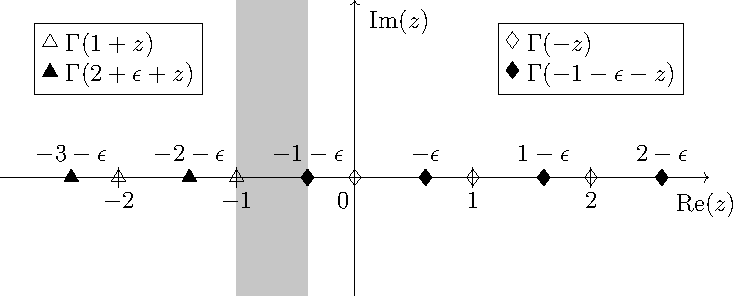
\includegraphics[scale=0.7]{ch4_loopints/figures/mellin_barnes_box.pdf}
\centering
\caption{Poles of the $\Gamma$ functions involved in the Mellin-Barnes parameterisation of the one-loop box integral~(\ref{eq:MBboxM}) assuming $-1<\eps<0$. For the integration in eq.~(\ref{MBbox}) to be well defined, the real part of $z$ must lie in the shaded area, between the right-most pole of the $\Gamma$ functions of the type $\Gamma(z+\ldots)$ and the left-most pole of those of the type $\Gamma(-z+\ldots)$.
}
\label{fig:box_MB}
\end{figure}


\subsection{Resolution of singularities in $\eps$}

Here we follow ref.~\cite{ch4Czakon:2005rk} and references therein.
We saw that the integral in \eqn{MBbox} is ill-defined for $\eps = 0$.
This can be traced back to the presence of the Gamma functions
$\Gamma(1+z)$ and $\Gamma(-1-\eps-z)$. The contour for the $z$ integration has to pass between the poles of these Gamma functions, which is only possible for $\eps<0$. In other words, as $\eps$ goes to $0$, the shaded area in fig.~\ref{fig:box_MB} is pinched between the right-most pole of $\Gamma(1+z)$ and the left-most pole of $\Gamma(-1-\eps-z)$. Before we can take the limit $\eps \to 0$, we must therefore deform the integration contour for $z$, so that it does not become pinched when taking the limit.
Let us deform the contour to the right.
This leads to a contribution of the residue at $z=-1-\eps$. In other words, 
\begin{align}
F_{4} = - \oint_{z=-1-\eps}  \frac{\d z}{2 \pi \i} \,  M(s,t,z;\eps) +  \int_{  \Re(z) = c }  \frac{\d z}{2 \pi \i} \, M(s,t,z;\eps) \,,
\end{align}
where $-1-\eps < c < 0$.
The value of this residue is
%
\begin{align} \label{eq:MBboxA}
A = \frac{ \left(-s\right)^{-{\eps}} }{s \, t} 
\frac{ \Gamma^2(-{\eps}) \Gamma ({\eps}+1) }{ \Gamma (-2
   {\eps})}
  \left[ 2 \, \psi(-{\eps})-\psi({\eps}+1)+\log\left(\frac{s}{t}\right)+\gamma_{\rm E} \right]\,,
\end{align}
where $\psi(z)$ is the digamma function, defined in \eqn{eq:psidef} of exercise~\ref{Ex:TaylorLogGamma}.

In the second term, we can safely Taylor expand in $\eps$.
We see that it is of $\cO(\eps)$, due to the presence of the factor $\Gamma(-2\eps)$ in the denominator. 
Here we keep only this leading term,
\begin{align} \label{eq:MBboxB}
B = -2 \eps \int_{  \Re(z) = c}  \frac{\d z}{2 \pi \i} \, \frac{1}{t^2} \left(\frac{s}{t}\right)^z  \Gamma(-z) \Gamma(2+z) {\Gamma^2(1+z) \Gamma^2(-1-z)}
  + \cO(\eps^2) \,,
\end{align}
where $-1<c<0$.
Therefore, remembering that the residue $A$ in \eqn{eq:MBboxA} contributes with a minus sign, we find
\begin{align}\label{eq:answerboxchapter4}
\mathrm{e}^{\eps \gamma_{\rm E}} F_{4} =  \frac{(-t)^{-\eps}}{s\,t} \left[  \frac{4}{\eps^2}  - \frac{2}{\eps}  \log \frac{s}{t} -  \frac{4 \pi^2}{3} + \cO(\eps)   \right] \,.
\end{align}
In exercise~\ref{Ex:4.BoxMellinBarnes} we compute also the $\cO(\eps)$ term.

\begin{svgraybox}
{\bf The full $--++$ helicity QCD amplitude.}
In chapter~\ref{ch:loopamps}, the one-loop four-gluon amplitude in the $++--$ helicity configuration was given in \eqn{eq:full_split_helicity_four_gluon_one_loop_integrand} in terms of box and bubble Feynman integrals.
Let us denote the ratio of the one-loop and the tree amplitude by
\begin{align}
 \mathrm{e}^{-\eps \gamma_{\rm E}}  \frac{\alpha_{\rm YM}}{(4 \pi)^{2-\eps}} M_{--++}^{(1)} \coloneqq  \frac{ A^{(1),[4-2\eps]}(1^-,2^-,3^+,4^+) }{A^{(0)}(1^-,2^-,3^+,4^+) }\,. 
\end{align}
%
Using the results for the integrals from eqs.~\eqref{eq:answerboxchapter4} and~\eqref{eq:Ibubblechapter4},
we find
\begin{align}\label{eq:finalresultQCDamplitude}
 M_{--++}^{(1)} =
&  - \frac{4}{\eps^2} +\frac{1}{\eps} \left[ -\frac{11}{3} +2  \log\left(- \frac{s}{\mu_{\rm R}^2} \right) + 2  \log\left(-\frac{t}{\mu_{\rm R}^2}\right) \right]   \\
&\hspace{-1cm}- 2  \log\left(-\frac{s}{\mu_{\rm R}^2}\right) \log\left(-\frac{t}{\mu_{\rm R}^2}\right) + \frac{4}{3}\pi^2  + \frac{11}{3} \log\left(-\frac{t}{\mu_{\rm R}^2}\right) - \frac{64}{9}  + {\cal O}(\eps) \nonumber
\,.
\end{align}
Here we have reinstated the dimensional regularisation scale $\mu_{\rm R}^2$.
We can rewrite this in the following instructive form,
\begin{align} \label{eq:finalresultQCDamplitude2}
\begin{aligned}
M_{--++}^{(1)}  =
& - \frac{2}{\eps^2}  \left(-\frac{s}{\mu_{\rm R}^2}\right)^{-\eps} - \frac{2}{\eps^2}  \left(-\frac{t}{\mu_{\rm R}^2}\right)^{-\eps} + \log^2 \left(\frac{s}{t}\right) +  \frac{4 \pi^2}{3}  \\
& \hspace{1cm}- \frac{11}{3 \eps}  + \frac{11}{3} \log\left(-\frac{t}{\mu_{\rm R}^2}\right) - \frac{64}{9} + {\cal O}(\eps) \,.
\end{aligned}
\end{align}
The special form of the poles in $\eps$ in \eqn{eq:finalresultQCDamplitude2} is related to the structure of ultraviolet and infrared divergences in Yang-Mills theories. 
It is due to the fact that ultraviolet and infrared effects come from separate regions. 
For an introduction to infrared divergences in Yang-Mills theories, see e.g.\ ref.~\cite{ch4Agarwal:2021ais}. 
\end{svgraybox}


\begin{exer}{Massless one-loop box with Mellin-Barnes parametrisation}
\label{Ex:4.BoxMellinBarnes}
Compute the order-$\eps$ term of the function $B$ in \eqn{eq:MBboxB}. Putting the latter together with the Laurent expansion of the residue $A$ in \eqn{eq:MBboxA} gives the analytic expression of the massless one-loop box integral $F_4$ up to order $\eps$:
%
\begin{align}  \label{eq:F4final}
\begin{aligned}
F_4 = \ & \frac{\text{e}^{-\epsilon \gamma_{\text{E}}} (-s)^{-\epsilon}}{s \, t} \biggl\{ \frac{4}{\eps^2} - \frac{2}{\eps} \log(x) -\frac{4 \pi^2}{3} +
  \epsilon \biggl[  2 \, \text{Li}_3\left(-\frac{1}{x}\right) + 
 2 \log(x) \, \text{Li}_2\left(-\frac{1}{x}\right)    \\
& + \log^3(x) + \frac{7 \pi^2}{6} \log(x) - \bigl(\log(x)^2+ \pi^2 \bigr) \log(1 + x)  - \frac{34}{3} \zeta_3 \biggr] + \mathcal{O}\bigl(\epsilon^2\bigr) \biggr\} \,,
\end{aligned}
\end{align}
where $x=t/s>0$. In this result we see for the first time the \emph{polylogarithm} $\mathrm{Li}_n(x)$, a special function which arises frequently in the computation of Feynman integrals. 
For $|x|<1$, the $n$-th polylogarithm ${\rm Li}_{n}(x)$ is defined as the power series
\begin{align}\label{def_polylogarithm_series}
{\rm Li}_{n}(x) \coloneqq \sum_{k\ge1 }\frac{x^k}{k^n} \,,\quad \quad {n=1,2,\ldots} \,.
\end{align}
The definition can be extended to the rest the complex plane by analytic continuation, e.g.\ by viewing the polylogarithms as solutions to differential equations. We will take this viewpoint in section~\ref{ref:subsection:propertiesofspecialfunctions}.
Note that the first polylogarithm is just a logarithm: ${\rm Li}_{1}(x) = - \log(1-x)$. The second polylogarithm, $\mathrm{Li}_2$, is typically referred to as \emph{dilogarithm}. At unit argument, the polylogarithms with $n\ge 2$ evaluate to Riemann's zeta constants: $\mathrm{Li}_n(1) = \zeta_n$.
%
For the solution see \hyperref[Sol:4.BoxMellinBarnes]{chapter~5}.

\end{exer}



\section{Special functions, differential equations, and transcendental~weight}
\label{ref:subsection:propertiesofspecialfunctions}


 \subsection{A first look at special functions in Feynman integrals}
 

In the previous section, we have already seen a few examples of special functions appearing in Feynman integrals,
namely the logarithm and the polylogarithm. We have also encountered special numbers: powers of $\pi$, as well as other transcendental constants such as $\zeta_3$.
The latter appear on their own, or arise as special values of the special functions, as we see presently.

These transcendental numbers and functions are ubiquitous in quantum field theory. For example, they may appear in anomalous dimensions of local operators, in the $\beta$ function governing the renormalisation group flow, or in scattering amplitudes. 
From a structural viewpoint it is very interesting to ask: what transcendental numbers may arise in a given computation?
Some of the techniques discussed later in this chapter came together from insights into this and related questions.

A first useful concept is the notion of \emph{transcendental weight}, or ``transcendentality''.
Roughly speaking, it describes the complexity of an expression. Rational numbers are assigned weight zero, while $\pi$ is assigned weight one, and more generally $\zeta_n$ is assigned weight $n$.
Likewise, the logarithm is assigned weight one, while the polylogarithm ${\rm Li}_n$ is assigned weight $n$.
The first interest in this definition came from two observations. Firstly, in the special ${\mathcal{N}}=4$ super Yang-Mills theory, quantities appear to always have a fixed, uniform weight. Secondly, for certain anomalous dimensions in QCD, which are not uniform in weight, the highest-weight piece agrees with the one computed in ${\mathcal{N}}=4$ super Yang-Mills theory~\cite{ch4Kotikov:2002ab}. These first observations stimulated more research that eventually led to a better understanding of transcendental weight, which allows one to predict which Feynman integrals have the maximal weight property. This insight is  useful for computing Feynman integrals, as we will discuss below.

We have seen a definition of the polylogarithm in \eqn{def_polylogarithm_series}. 
There are many examples of special functions in physics, and usually there exist several equivalent definitions.
The same is the case here. 
In many cases, a definition in terms of a defining differential equation is convenient.
We will follow this approach in this section, and will discover that it is very useful in the context of Feynman integrals.
Therefore let us first review the functions we encountered so far from this perspective, which is closely related to integral representations, and discuss some of their key~properties.

The logarithm can be defined as a single integral: 
\begin{align}\label{eq:logxreal}
\log x = \int_{1}^{x} \frac{\d t}{t} \,.
\end{align}
This equation is defined for real positive $x$. 
To extend the definition to complex argument, one places a branch cut along the negative real axis, and defines the answer in the cut complex plane by analytic continuation, i.e.\ by integrating along a contour from the base point $x=1$ to the argument $x \in \mathbb{C} \setminus \{x<0\}$, as shown in fig.~\ref{fig:logarithm}.

\begin{figure}[t]
\centering
\begin{tikzpicture}[baseline={(current bounding box.center)}, scale =1.0,
  decoration={markings,  mark= at position 0.5 with {\arrow{stealth}}}]
  % draw horizontal axis
  \draw[->] (-2.5,0) -- (2.5,0) node[below] {${\rm Re}(x)$};
  % draw vertical axis
  \draw[->] (0,-0.5) -- (0,2) node[left] {${\rm Im}(x)$};
  % draw dot at x=1
  \node[below right] at (0,0) {$0$};
  \filldraw (1,0) circle (2pt) node[below right] {$1$};
    % draw horizontal zigzag line
    \draw[decorate,decoration={zigzag,segment length=4pt}] (-2.5,0) -- (0,0);
       % draw curvy line with two swings
    \draw[postaction={decorate}] (1,0) .. controls (1.5,2.5) and (-0.5,0.5) .. (-1.5,1);
      % draw dot not filled
      \draw (-1.5,1) circle (2pt) node[below left] {$x$};
      \end{tikzpicture}
   \caption{Integration contour to extend the definition of the logarithm to the complex plane with the branch cut along the negative real axis removed, as indicated by the zig-zag line.}
  \label{fig:logarithm}
\end{figure}

From \eqn{eq:logxreal} we can simply read off the derivative,
\begin{align}\label{eq:difflog}
\partial_x \log x &= \frac{1}{x} \,,
\end{align}
and we have $\log 1 = 0$.
Dilogarithms can be defined in a similar way, but with two integrals instead of one:
\begin{align} \label{eq:Li2_integral}
{\rm Li}_{2}(x) = - \int_{0}^{x} \frac{\d t}{t} \log(1-t) \,.
\end{align}
One may verify that this agrees with the series representation~\eqref{def_polylogarithm_series} by Taylor expanding the integrand in $t$.
From this we can read off the derivatives,
\begin{align}
\partial_x {\rm Li}_{2}(x) &= -\frac{1}{x} \log(1-x) \,,\\
\partial_x {\rm Li}_{2}(1-x) &= \frac{1}{1-x} \log(x)  \label{diffeqLi2}  \,,
\end{align}
as well as the special value  ${\rm Li}_{2}(0) = 0$. Like the logarithm, the dilogarithm ${\rm Li}_2(x)$ is a multi-valued function. Its branch points are at $x=1$ and infinity. Following the convention of the logarithm, the branch cut is along the positive real axis between $x=1$ and infinity (see exercise~\ref{Ex:Discontinuities}).
For more information about the dilogarithm, see~\cite{ch4Zagier:2007knq}.

We have seen that this, as well as the trilogarithm encountered above, are part of a larger class of polylogarithms, defined in terms of series in \eqn{def_polylogarithm_series}.
 In the following, it will be useful to think of these functions in terms of iterated integrals.
 To establish the connection, we note that 
\begin{align}
x \, \partial_x {\rm Li}_{n}(x) &=  {\rm Li}_{n-1}(x) \,,\quad {\rm for} \;\; n>2 \,,
\end{align}
which follows straightforwardly from \eqn{def_polylogarithm_series}. 
Therefore we can write
\begin{align}
 {\rm Li}_{n}(x) = \int_0^x  {\rm Li}_{n-1}(y) \frac{\d y}{y}  \,,\quad {\rm for} \;\; n>2 \,.
\end{align}
All polylogarithms ${\rm Li}_{n}(x)$ are multi-valued functions, with a branch cut along the positive real axis between $x=1$ and infinity.
Note that we can think of all those functions as iterated integrals over certain logarithmic integration kernels: $\d x/x$ and $\d x/(x-1)$.
This leads to another way to think about transcendental weight: it corresponds to the number of integrations in such an iterated-integral representation.



\begin{exer}{Discontinuities}
\label{Ex:Discontinuities}
The discontinuity of a univariate function $f(x)$ across the real $x$ axis is defined~as
\begin{align}
\mathrm{Disc}_x \left[f(x)\right] \coloneqq \lim_{\eta\to 0^+} \left[ f(x+\i \eta) - f(x- \i \eta) \right] \,.
\end{align}
\begin{enumerate}[a)]
\item Prove that the discontinuity of the logarithm is given by
\begin{align} \label{eq:disc_log}
\mathrm{Disc}_x \left[\log(x)\right] = 2 \pi \i \, \Theta(-x) \,,
\end{align}
where $\Theta$ denotes the Heaviside step function. 

\smallskip
\item The dilogarithm ${\rm Li}_2(x)$ has a branch cut along the real $x$ axis for $x>1$. Prove that the discontinuity is given by
\begin{align} \label{eq:disc_dilog}
\mathrm{Disc}_x \left[\text{Li}_2(x)\right] = 2 \pi \i \, \log(x) \, \Theta(x-1) \,.
\end{align}
Hint: use the identity
\begin{align} \label{eq:Li2identity}
{\rm Li}_2(x) = - {\rm Li}_2(1-x) - \log(1-x) \log(x) + \zeta_2 \,,
\end{align}
which we shall prove in exercise~\ref{Ex:4.W2basis}.

\end{enumerate}
For the solution see \hyperref[Sol:Discontinuities]{chapter~5}.
\end{exer}




\subsection{Special functions from differential equations: the dilogarithm}
\label{sec:sepcialfunctionsfromDE}

Let us now see how we can think of these functions conveniently from a differential equations approach. 
Say we are interested in the function ${\rm Li}_{2}(1-x)$, perhaps because we know that it can appear in a certain calculation.
Our goal is to find a defining set of differential equations for this function. Inspecting \eqn{diffeqLi2}, we see that $\log(x)$ appears in its derivative, so we consider this function also, as well as the constant $1$, which is required to write the derivative of $\log(x)$. 
Let us put these key functions into a vector,
\begin{align} \label{definitionfLi2}
\vec{f}(x)= \begin{pmatrix} {\rm Li}_{2}(1-x) \\ \log(x) \\ 1 \end{pmatrix}
\,.
 \end{align}
 A short calculation then shows that the following differential equation is satisfied,
  \begin{align} \label{exampleDELi2matrix2}
\partial_x \vec{f}(x)=  \left( \frac{A_0}{x}  +  \frac{A_1}{x-1} \right) \cdot \vec{f}(x)
\,.
 \end{align}
with the matrices
 \begin{align} \label{exampleDELi2matrix}
A_0 = {\begin{pmatrix}0 & 0 & 0 \\ 0 & 0 & 1 \\ 0 & 0 & 0 \end{pmatrix}}  \,, \quad  A_1 = {\begin{pmatrix}0 & -1 & 0 \\ 0 & 0 & 0 \\ 0 & 0 & 0 \end{pmatrix}}\,.
 \end{align}
The first-order differential equations~\eqref{exampleDELi2matrix2}, together with the boundary condition $\vec{f}(x=1) = (0,0,1)^{\top}$, uniquely fix the answer.

Equation~\eqref{exampleDELi2matrix2} encodes the singular points $x=0,1,\infty$ of the functions. As we will see later, the leading behaviour of $\vec{f}(x)$ is governed by the coefficient matrices of those singular points, which are $A_0,A_1,A_{\infty}=-A_0-A_1$, respectively.
The last point can be understood by changing variables to $y=1/x$, and inspecting the singularity at $y=0$.

Let us now see how this connects to the concept of transcendental weight.
Recall that, when referring to iterated integrals, the weight counts the number of integrations. So the rational constant has weight zero, a logarithm has weight one, the dilogarithm has weight two, and so on.
Looking at \eqn{definitionfLi2}, we see that the different components of $\vec{f}$ have different weight. 
In order to remedy this, we introduce a weight-counting factor $\eps$, to which we assign the weight $-1$~\cite{ch4Henn:2013pwa}.
For the moment, this is a purely formal definition. However, later we will see that this is natural in the context of dimensional regularisation.\footnote{In particular, poles $1/\eps$ in dimensional regularisation correspond to $\log \Lambda$ terms in cutoff regularisations, so it is natural that $1/\eps$ has the same weight as a logarithm.} 
With the weight-counting parameter $\eps$ at our disposal, we can define
\begin{align} \label{eq:defg}
\vec{g}(x;\eps)= \begin{pmatrix} \eps^2 {\rm Li}_{2}(1-x) \\ \eps \log(x) \\ 1 \end{pmatrix}
\,.
 \end{align}
This vector has uniform weight zero by definition. 
We find that it satisfies the following differential equations:
 \begin{align}\label{eqDEgLi2canonical0}
 \partial_x \vec{g}(x;\eps) = \eps \left( \frac{A_0}{x} + \frac{A_1}{x-1} \right) \cdot \vec{g}(x;\eps) \,.
 \end{align}
It is instructive to rewrite this in differential form, as
\begin{align}\label{eqDEgLi2canonical}
\d \, \vec{g}(x;\eps) = \eps \bigl[ A_0\, \d \log(x) + A_1\, \d \log(1-x) \bigr] \cdot \vec{g}(x;\eps) \,,
\end{align}
 where $\d= \d x \frac{\partial}{\partial x}$.
 We can see that the weights in this equation are consistent:
 $\d$ and $\eps$ have weight $-1$, $\log$ has weight $+1$, and the constant matrices $A_0$ and $A_1$ have weight zero. 
  Therefore $g$ has weight zero. 
  Since $g$ depends on $\eps$, this means that when expanding in a series around $\eps=0$, the weight of the coefficients increases with the order in $\eps$, starting with weight zero at order $\eps^0$.
  This is of course exactly what is expected from \eqn{eq:defg}.
  
 Let us now see how this arises from solving \eqn{eqDEgLi2canonical}. Plugging the ansatz
 \begin{align}
\vec{g}(x;\eps) = \sum_{k \ge 0} \eps^k \vec{g}^{(k)}(x) 
 \end{align}
into the DE, and looking at the different orders in $\eps$, we see that the equations decouple. The first few orders read 
\begin{align}\label{eq:DEgexpanded}
 & \partial_x \vec{g}^{(0)}(x) = 0 \,, \\
 &  \partial_x \vec{g}^{(1)}(x) = A(x) \cdot \vec{g}^{(0)}(x)\,,\\
 &  \partial_x \vec{g}^{(2)}(x) = A(x) \cdot \vec{g}^{(1)}(x) \,,
\end{align}
at order $\eps^{0}, \eps^{1}, \eps^{2}$, respectively, and so on.
Recalling the boundary condition $\vec{g}(1,\eps) = (0,0,1)^{\top}$,
the equations are readily solved, giving
 \begin{align}
 \vec{g}^{(0)}(x) = 
 \begin{pmatrix} 0 \\ 0 \\ 1 \end{pmatrix}\,,\quad
 \vec{g}^{(1)}(x) = 
 \begin{pmatrix} 0 \\ \log x \\ 0 \end{pmatrix}\,,\quad
\vec{g}^{(2)}(x) =
  \begin{pmatrix} {\rm Li}_{2}(1-x) \\ 0 \\ 0 \end{pmatrix}\,.
 \end{align}
 The higher-order equations read $ \partial_x \vec{g}^{(3)}(x) = A(x) \cdot \vec{g}^{(2)}(x)  =0 $, which lead to $\vec{g}^{(3)}(x) = (0,0,0)^{\top}$, and similarly at higher orders. In other words, the $\eps$ expansion stops at $\eps^2$. The reason is that, in this specific case, $A(x)$ is a nilpotent matrix, i.e., $A(x)^3 = 0$. 
This will be different for general Feynman integrals in $D=4-2\eps$ dimensions, but it will not limit the usefulness of the method.

\begin{important}{It is useful to think about special functions in terms of their defining differential equations.}
Just as in familiar textbook examples from quantum mechanics, differential equations turn out to be a useful
 way of {\it defining} classes of special functions. We shall see later in this chapter that this strategy is particularly effective for Feynman integrals.
\end{important}
 
\subsection{Comments on properties of the defining differential equations}
 \label{subsec:comments}

Let us make a number of important comments on the differential equations~\eqref{eqDEgLi2canonical} discussed in the last subsection.

\smallskip

1. {\it  Fuchsian nature of the singularities}. Equation~\eqref{eqDEgLi2canonical} has several special features. 
One of them is the nature of its singularities. We see that the matrices on its RHS have only simple poles at each singular point. 
It implies that the asymptotic solution near any singular limit, say $x\to 0$, can be expressed in terms of powers of $x$ and logarithms of $x$.
This type of singularity is called Fuchsian.
In contrast, consider differential equations with a non-Fuchsian singularity, e.g.
\begin{align} \label{eq:DEnonFuchsian}
\partial_x f(x) = \frac{a}{x^2} \, f(x) \,.
\end{align}
The solution to \eqn{eq:DEnonFuchsian} reads 
\begin{align}
f(x) = \mathrm{e}^{-a/x} f_0\,,
\end{align} 
for some boundary constant $f_0$. This has non-analytic behaviour at $x=0$, which is not expected from individual Feynman integrals. 


We will see in section~\ref{sec:DEFeynmanintegrals} that the Fuchsian property is useful in several regards. Firstly, it may help in finding simple forms of the differential equations.
Secondly, analysing the behaviour of the equations near singular points provides crucial information for fixing integration constants based on physical principles, without additional calculations~\cite{ch4Henn:2020lye}.
Thirdly, the asymptotic expansion of an integral in a certain limit can be read off easily from the differential equations. 


\smallskip

2. {\it  ``Gauge dependence'' of the differential equations}. 
The differential equations 
\begin{align}\label{eq:generalDEincommentsection}
\partial_x \vec{f}(x,\eps) = A(x,\eps) \cdot \vec{f}(x,\eps)
\end{align}
 are not unique in the following sense. 
Consider an invertible matrix $T(x,\eps)$, such that we can define the following change of basis,
\begin{align} \label{eq:gaugetransformation}
\vec{f} = T \cdot \vec{g} \,.
\end{align}
Then the new basis $\vec{g}$ satisfies similar differential equations, $\partial_x \vec{g} = B \cdot \vec{g}$, with a different matrix
\begin{align}\label{eq:defB}
B = T^{-1} \cdot A \cdot T - T^{-1} \cdot \partial_x T \,.
\end{align}
Note that the ``connection matrix'' $A$ transforms to $B$ as under a gauge transformation.



For this reason, even if a simple form of the differential equations such as \eqn{eqDEgLi2canonical} exists, this fact might be obscured if an unfortunate choice of basis is made. 
In particular, the Fuchsian property mentioned above may be obscured in this way.
However, a judicious basis choice can reveal the simplicity of the answer.

For example, consider the following matrix,
\begin{align}
T=  {\begin{pmatrix} 1+x & 0 & 1 \\ 1 & -x & 0 \\ 0 & 0 & 1  \end{pmatrix}} \,,\quad {\rm with} \quad T^{-1} = {\begin{pmatrix} \frac{1}{1+x} & 0 & -\frac{1}{1+x} \\ \frac{1}{x (1+x)} & -\frac{1}{x} & -\frac{1}{x (1+x)} \\ 0 & 0 & 1  \end{pmatrix}} \,.
\end{align}
Applying this to $A= A_0/x + A_1/(x-1)$ with~\eqref{exampleDELi2matrix}, we find that \eqn{eq:defB} evaluates~to
\begin{align}
B = {\begin{pmatrix} \frac{1-\eps-x}{(x-1)(x+1)} & \frac{\eps x}{(x-1)(x+1)} & 0 \\ \frac{1-\eps-x}{(x-1)(x+1)x} & \frac{1+\eps x-x^2}{(x-1)(x+1)x} & -\frac{\eps}{x^2}  \\ 0 & 0 & 0  \end{pmatrix}} \,.
\end{align}
This new form of the DE is far worse compared to the original one, for three reasons. First, the factorised $\eps$-dependence is lost. Second, there is a spurious divergence at $x=-1$. Third, the Fuchsian property at $x=0$ is no longer manifest, due to the $1/x^2$ term. This example underlines the importance of good guiding principles when dealing with this type of differential equations.

\smallskip

3.  {\it  Solution as a path-ordered exponential}. 
The analogy with gauge transformations mentioned in point~2 above allows us to write down the solution to the general differential equations~\eqref{eq:generalDEincommentsection}. 
The latter
is given by the following expression 
\begin{align}\label{eq:Wilsonlinesolution}
\vec{f}(x) = {\mathbb P} \exp\left[ \int_{\cal C} A(x') \d x' \right]  \cdot \vec{f}(x_0) \,.
\end{align}
Here ${\cal C}$ is a path connecting the \textit{base point} $x_{0}$ to the function argument $x$,
 ${\mathbb P}$ stands for path ordering along this path, and $f(x_{0})$ is the value of the function at the base~point.


In the formal expansion of the matrix exponential appearing in \eqn{eq:Wilsonlinesolution}, the arguments are evaluated at different points $x'$ along the path ${\cal C}$. In practice, one may consider the pull-back of the form $A(x') \d x'$ to the unit interval, parametrised by a parameter $t\in [0,1]$. 
The path-ordering then dictates that the matrices are ordered according to the ordering on the unit interval.


Equation~\eqref{eq:Wilsonlinesolution} may be familiar to readers. On the one hand, the path ordering also shows up as time-ordering in the evolution operator in quantum mechanics. On the other hand, somewhat more advanced, it shows up in gauge theory: given a gauge field $A$, the matrix  $ {\mathbb P} \exp\bigl[ \int_{\cal C} A(x') \d x' \bigr]$ represents a Wilson line connecting two points $x_0$ and $x$, along a contour ${\cal C}$. 

This second analogy also makes it clear that \eqn{eq:Wilsonlinesolution} enjoys a manifest {\it homotopy invariance}: two contours ${\cal C}$ and ${\cal C'}$ (connecting $x$ and $x_0$) give the same value, as long as they can be smoothly deformed into each other, without crossing poles of $A$.

For general $A$, the RHS of \eqn{eq:Wilsonlinesolution} is somewhat formal. However, in the cases considered  in these lectures, it can be made very explicit. Firstly, in the dilogarithm example of section~\ref{sec:sepcialfunctionsfromDE}, $A$ is nilpotent, and hence the path-ordered exponential has a finite number of terms (and hence number of iterated integrals) only. Secondly, in a later section we propose a method that achieves that $A \sim \eps$, which allows us to write the path-ordered exponential as a Taylor series in $\eps$. This is analogous to a perturbative expansion in the Yang-Mills coupling in gauge theory.

\smallskip

\begin{figure}[t]
\centering
\begin{tikzpicture}[baseline={(current bounding box.center)}, scale =1.0, 
   decoration={markings,  mark= at position 0.56 with {\arrow{stealth}}}]
  % draw horizontal axis
  \draw[->] (-2.5,0) -- (2.5,0) node[below] {${\rm Re}(x)$};
  % draw vertical axis
  \draw[->] (0,-1) -- (0,2) node[left] {${\rm Im}(x)$};
  % draw dot at x=1
  \node[below right] at (0,0) {$0$};
  \filldraw (1,0) circle (2pt) node[below right] {$1$};
    % draw horizontal zigzag line
    \draw[decorate,decoration={zigzag,segment length=4pt}] (-2.5,0) -- (0,0);
       % draw curvy line with two swings
    \draw[postaction={decorate}] (1,0) .. controls (1.5,2.5) and (-0.5,0.5) .. (-1.5,1);
    \node at (1.15,1.2) {$\mathcal{C}$};
       % draw another curvy line with two swings
    \draw[postaction={decorate}]  (1,0) .. controls (-1.5,-1.5) and (-0.5,-0.5) .. (-1.5,1);
    \node at (-1.,-0.8) {$\mathcal{C}'$};
      % draw dot not filled
      \draw (-1.5,1) circle (2pt) node[below left] {$x$};
      \draw[mark=x, mark size=4pt,thick] plot (0,0);
      \draw[mark=x, mark size=4pt,thick] plot (1,0);
      \end{tikzpicture}
   \caption{
   Integration contours for solving the defining DE of the dilogarithm $\mathrm{Li}_2(1-x)$, eq.~(\ref{exampleDELi2matrix2}). The zig-zag line denotes the branch cut, and the crosses the poles of the connection matrix. The difference between integrating the DE along the two contours gives the discontinuity of the solution.}
  \label{fig:logarithm_disc}
\end{figure}

4. {\it Discontinuities} (see exercise~\ref{Ex:Discontinuities}) are also solutions to the differential equations. 
This is obvious from the form~\eqref{eq:Wilsonlinesolution} of the general solution.
Indeed, consider two contours ${\cal C}$ and ${\cal C'}$ that differ by a contour encircling a pole of $A$. 
Since both  ${\cal C}$ and ${\cal C'}$ are solutions to \eqn{eq:generalDEincommentsection}, so is their difference.
The latter corresponds to taking a discontinuity of $\vec{f}$.
For instance, in our example above (\eqn{exampleDELi2matrix2}), we may consider two contours $\mathcal{C}$ and $\mathcal{C}'$ as in figure~\ref{fig:logarithm_disc}, with $\mathcal{C}'$ crossing the branch cut starting from $x=0$. In this case, for $x\in \mathbb{C} \setminus \{x<0\}$, we find~that
\begin{align} \label{eq:disc_example}
\begin{aligned}
{\rm Disc}_{x=0} \, \vec{f}(x) & = \left\{ \mathbb{P} \, \mathrm{exp}\left[\int_{\mathcal{C}} A(x') \d x' \right] - \mathbb{P} \, \mathrm{exp}\left[\int_{\mathcal{C}'} A(x') \d x' \right] \right\} \cdot \vec{f}(x_0) \\
 & = 2 \pi \i \, \begin{pmatrix}  -\log(1-x) \\ 1 \\ 0 \end{pmatrix} \,,
\end{aligned}
\end{align}
which is equally a solution to \eqn{exampleDELi2matrix2}. This way of defining the discontinuity is more general than the one we have seen in exercise~\ref{Ex:Discontinuities} and chapter~\ref{ch:loopamps}---which was restricted to the real axis---and is more suitable to functions involving multiple branch points.\footnote{In fact, note that the connection matrix in the DE~\eqref{exampleDELi2matrix2} has a pole also at $x=1$. This branch point is ``hidden'' in the principal branch of $\mathrm{Li}_2(1-x)$, but comes to light when we cross the branch cut starting from $x=0$. Indeed, we see in \eqn{eq:disc_example} that the discontinuity of $\mathrm{Li}_2(1-x)$ has itself a branch point at $x=1$.} For this reason we indicate the branch point in the subscript of the discontinuity in \eqn{eq:disc_example}. 
This property of the discontinuity will be useful when analysing Feynman integrals.



\smallskip

5. {\it Relation to   Picard-Fuchs equation}. The issue raised in the previous point can be addressed in part in the following way. We can trade the first-order system of differential equations for higher-order equations for one of the integrals, called Picard-Fuchs equations~\cite{ch4Muller-Stach:2012tgj}. 
Let us illustrate this for the ${\rm Li}_{2}(1-x)$, which is the first component of ${\bf f}$ in \eqn{definitionfLi2}. Differentiating $\vec{f}$ multiple times with the help of \eqn{exampleDELi2matrix2}), one obtains a system of equations, from which one eliminates all functions except $\vec{f}_{1}$ and its derivatives.
In the present case we get 
\begin{align}
\partial_x x \partial_x (1-x) \partial_x {\rm Li}_{2}(1-x) = 0\,.
\end{align}
An advantage of this representation as compared to \eqn{eqDEgLi2canonical} is that it depends only on one function, ${\rm Li}_{2}(1-x)$, and not on the other elements in the vector ${\bf f}$. As such it does not suffer from the gauge dependence mentioned~above. 

\smallskip

6. {\it Dependence on the weight-counting parameter $\eps$}.
Recall that we assigned to $\eps$ transcendental weight $-1$.
We saw that when each $w$-fold iterated integral appearing in the basis $\vec{f}$ was multiplied by a factor $\eps^w$, then the differential equations had a simple, factorised dependence on $\eps$, cf.~\eqn{eqDEgLi2canonical}. Conversely, had we considered linear combinations of mixed weight, or had we not normalised the integrals appropriately, the dependence on $\eps$ would have been more complicated. This is important to bear in mind when applying the above philosophy to Feynman integrals. 
 
 \smallskip 
 
 7. {\it Uniform weight functions and pure functions}.
 It turns out that the simplicity of the differential equations considered in this chapter can be easily understood. For this it is useful to introduce the following concepts. A {\it uniform weight} function is a linear combination of functions of some uniform weight $w$, with coefficients that may be rational or algebraic functions. An example is 
 \begin{align}
  \frac{1}{1+x} {\rm Li}_{2}(1-x)  + \frac{x}{1-x} \log^2(1+ x) \,.
 \end{align}
 Such a function does not satisfy particularly nice differential equations. The reason is that a derivative $\partial_x$ can act either on one of the prefactors, or on the transcendental functions. As a result, one obtains a function of mixed transcendental weight. In contrast, consider a {\it pure function}, which is a ${\mathbb Q}$-linear combination of functions of some uniform weight $w$. An example for $w=2$ is
 \begin{align}
 {\rm Li}_{2}(1-x)  +  \log^2(1+ x) \,.
 \end{align} 
 Its derivative is
 \begin{align}
 \frac{1}{1-x} \log x + \frac{2}{1+x} \log(1+x) \,,
 \end{align}
 which has weight one, i.e.\ one less than the original function.
It is built from two new pure functions, for which we could iterate the differential procedure. In this way one can construct a system of differential equations similar to the one considered above for any pure function. This also generalises naturally to multi-variable functions.
 

 




\subsection{Functional identities and symbol method}
 \label{sec:functionalidentitiesandsymbolmethod}
 
We will see that the key properties of the special functions can be encoded in so-called {\it symbols}. Roughly speaking, symbols preserve the information on the integration kernels but disregard the integration constants. 
In this context, the integration kernels are called \emph{letters}, and their ensemble \emph{alphabet}. 
For example, the alphabet associated with the DE~\eqref{eqDEgLi2canonical} has two letters: $\d \log(x)$ and $\d \log(1-x)$.\footnote{Whenever the alphabet contains only $\d \log$-type integration kernels, it is sufficient to keep track of their arguments. In the case of \eqn{eqDEgLi2canonical}, for instance, one would say that the alphabet is $\{x,1-x\}$.}
Concatenating different alphabet letters into words corresponds to specific iterated integrals. Leveraging the basic addition identity of the logarithm, the symbol technique allows one to detect function identities by simple algebra. 

Consider as an example the following function,
\begin{align}\label{defgexamplesymbol}
g(x) \coloneqq {\rm Li}_{2}(x) + {\rm Li}_{2}\left(\frac{1}{x}\right) + \frac{1}{2} \log^2(-x) + \frac{\pi^2}{6} \,. 
\end{align}
Let us consider this for $x<0$, such that we stay away from branch cuts, and all summands are real-valued.
We now wish to show that $g(x) =0$.
It is instructive to do this in the most elementary way, namely to show that $g'(x) =0$, and that the identity is true at some value of $x$.
Using \eqn{diffeqLi2} we have
\begin{align}
x \, \partial_x g(x) = - \log(1-x) + \log\left(1- \frac{1}{x} \right) + \log(-x)  = 0 \,.
\end{align}
In the last step, we have assumed $x<0$, so that we can use $\log(a b) = \log(a) + \log(b)$ for $a,b>0$.
Moreover, using ${\rm Li}_{2}(-1) = -\pi^2/12$, one verifies that $g(-1) = 0$. This completes the proof of the dilogarithm inversion identity $g(x)=0$.

The symbol method can streamline finding avatars of such identities, i.e.\ identities up to possibly integration constants.
It leverages the fact that we are dealing with iterated integrals, whose integration kernels satisfy the basic logarithm identity
\begin{align} \label{eq:dlogid}
\d \log(a b) = \d \log(a) + \d \log(b)\,.
\end{align}
Unlike the analogous identity for the logarithm, \eqn{eq:dlogid} holds for any non-vanishing $a$ and $b$, as $\d \log c = 0$ for any constant $c$.
Let us now see this in practice, first giving an intuitive explanation, and then a formal definition. Given an iterated integral, say 
\begin{align}
 {\rm Li}_{2}(x) 
 =&  -  \int_0^x \d\log(y) \int_0^y \d\log(1-z) \,, \label{Li2dlog} 
 \end{align}
we read off its logarithmic integration kernels, which are $\d\log(1-z)$ and $\d\log(y)$, respectively, and record their arguments in the symbol, denoted by square brackets,
 \begin{align}\label{eq:Li2symbolexample}
{\cal S} \bigl( {\rm Li}_{2}(x) \bigr) =& - [1-x,x] \,.
 \end{align}
 An alternative notation in the literature is $- (1-x) \otimes x$. We prefer the bracket notation to make it clear that the minus sign in \eqn{eq:Li2symbolexample} multiplies the symbol, rather than being one of its entries.
 
 Note that the order of integration kernels in the symbol $[\ldots ]$ is opposite to that in the integral representation,~\eqn{Li2dlog}.
 Readers might find confusing why the entries of the symbol in \eqn{eq:Li2symbolexample} depend on $x$, while in \eqn{Li2dlog} they depend on the (mute) integration variables. To clarify this, we find it best to give the following formal definition of the symbol.
 
 \smallskip
 
 {\it Recursive symbol definition for iterated integrals}. Let $f^{(w)}$ be a uniform 
  weight-$w$ function whose derivative is given by 
 \begin{align}\label{defsymbol1}
\d f^{(w)} = \sum_i c_i \, f_{i}^{(w-1)} \d\log \alpha_i\,,
\end{align}
where $c_{i}$ are kinematic-independent constants, $f_{i}^{(w-1)}$ are uniform weight-$(w-1)$ functions, and $\alpha_i$ are algebraic expressions depending on the kinematic variables.
 Then we define the symbol ${\cal S}$ of $f^{(w)}$ iteratively to be 
\begin{align}\label{defsymbol2}
\mathcal{S}\bigl(f^{(w)}\bigr) = \sum_i c_i  \bigl[ \mathcal{S}\bigl(f_{i}^{(w-1)} \bigr) , \alpha_i \bigr] \,.
 \end{align}
The iterative definition starts at weight $0$ with the ``empty'' symbol $[] \coloneqq \mathcal{S}(1)$. Applying this definition to the logarithm gives
\begin{align} \label{eq:symbol_log}
\mathcal{S}(\log x ) = [x] \,,
\end{align}
while for the dilogarithm we readily recover \eqn{eq:Li2symbolexample}.

\begin{exer}{The symbol of a transcendental function}
\label{Ex:4.Symbol}
Compute the symbol of $\log(x) \log (1-x)$.
For the solution see \hyperref[Sol:4.Symbol]{chapter~5}.
\end{exer}

Note that \eqn{defsymbol1}, and hence the definition of the symbol~\eqref{defsymbol2}, does not know about integration constants. 
In particular, constants such as $\pi^2/6$ in \eqn{defgexamplesymbol} are set to zero by the symbol map.
Moreover, since the definition is recursive, at weight $w$ the symbol in principle misses $w$ integration constants.
Nevertheless, the symbol is very useful: it provides a shortcut to discovering that an identity between transcendental functions exists. 
Let us now see how this works.

\smallskip

{\it Basic symbol properties}. It follows from the basic identity~\eqref{eq:dlogid} that the symbol satisfies
\begin{align} \label{eq:symbol_properties} \begin{aligned}
& [\ldots , a \, b , \ldots ] = [\ldots, a , \ldots ] +  [\ldots, b , \ldots ]\,, \\
& [\ldots , x^c , \ldots ] =c \, [\ldots, x , \ldots ]\,.
\end{aligned} \end{align}
Moreover, $[\ldots , c , \ldots ] = 0$ if $c$ is a constant.

Let us see how this works on $g(x)$ of \eqn{defgexamplesymbol}. We have
\begin{align}
{\cal S}\bigl({\rm Li}_{2}(x) \bigr) = \ & - [1-x,x] \,, \\
{\cal S}\left({\rm Li}_{2}\left(\frac{1}{x}\right)\right) = \ & - \left[1-\frac{1}{x},\frac{1}{x} \right] =  \left[- \frac{1-x}{x},x\right]  = [1-x,x]-[x,x]  \,, \\
{\cal S}\left(\frac{1}{2} \log^2(-x) \right) = \ &  [-x,-x] = [x,x]  \,, \\
{\cal S}\left(\frac{\pi^2}{6}\right) = \ & 0\,.
\end{align}
From this we readily conclude that the symbol identity ${\cal S}\bigl( g(x) \bigr) = 0$ holds.
What this means is the following.

\begin{important}{Symbols allow us to effortlessly find ``avatars'' of identities between transcendental functions.}
Finding a symbol identity implies a corresponding functional identity, with integration constants yet to be fixed. This can be done systematically. The ``beyond-the-symbol terms'' may in general involve constants times lower-weight functions.
\end{important}

\smallskip

{\it Connection between first and last entries to discontinuities and differentiation, respectively}.
%
By definition~\eqref{defsymbol1}, the last entry tells us how a symbol behaves under differentiation.
Interestingly, the first entry also has an important meaning: it is related to discontinuities.
Both these properties can be understood by thinking about symbols as iterated integrals.

For a logarithm $\log x$, the symbol is just $[x]$. Taking the discontinuity (normalised by $1/(2 \pi \i)$) across the negative real axis corresponds to replacing $[x] \to 1$.
Higher-weight functions are more interesting. For example, taking a discontinuity of $-[x,1-x]$, which is the symbol of ${\rm Li}_{2}(1-x)$, yields $-[1-x] = {\mathcal S}\bigl(- \log (1-x) \bigr)$.
For more details, see exercise~\ref{Ex:Discontinuities}.
In summary, we have that
\begin{align} \begin{aligned}
\d \, [a_1,\ldots,a_{n-1},a_n] & = \d \log(a_n) \times [a_1,\ldots,a_{n-1}] \,, \\
\mathrm{Disc} [a_1,a_2,\ldots,a_n] & = \mathrm{Disc}(\log a_1) \times [a_2,\ldots,a_n] \,.
\end{aligned} \end{align}
We thus see that, on top of providing a short-cut to finding functional relations, the symbol also encodes manifestly the branch-cut structure and the derivatives of the~functions.

\smallskip

{\it Function basis at weight two}. 
The symbol method is very useful when looking for simplifications, or when comparing results of different calculations.
In fact, for a given symbol alphabet (i.e., a given set of integration kernels), and up to a given weight, it is possible to classify the full space of possible functions.

Let us discuss this in more detail for the alphabet consisting of $\{x, 1-x \}$ that we are already familiar with. At weight two, there are four symbols we can build from these letters, namely 
\begin{align}\label{eq:symbolbasisweight2}
\bigl\{ [x,x] , [x,1-x], [1-x,x], [1-x,1-x] \bigr\} \,.
\end{align}
Once we write down a basis for this space, we can then rewrite any other weight-two function with those integration kernels in terms of that basis. 


\begin{exer}{Symbol basis and weight-two identities}
\label{Ex:4.W2basis}
%
\vspace{-0.6cm}
\begin{enumerate}[a)]
\item Verify that 
\begin{align} \label{eq:funcbasisW2}
\bigl\{ \log^2(x), \, \log^2 (1-x), \, \log(x) \log (1-x), \, {\rm Li}_{2}(1-x)\bigr\}
\end{align}
provides a basis for \eqn{eq:symbolbasisweight2}.
\smallskip
\item Compute the symbols of 
\begin{align} \label{eq:dilogs}
{\rm Li}_{2}(x) \,, \  {\rm Li}_{2}(1/x) \,, \  {\rm Li}_{2}\left(1/(1-x)\right) \,, \  {\rm Li}_{2}\left(x/(x-1)\right) \,, \ {\rm Li}_{2}\left((x-1)/x\right)  \,, 
\end{align}
and show that they ``live'' in the space spanned by the symbols in \eqn{eq:symbolbasisweight2}.  
\smallskip
\item Derive the identities (at symbol level) for rewriting the functions in point b in terms of the basis given in point a.
\end{enumerate}
For the solution see \hyperref[Sol:4.W2basis]{chapter~5}.
\end{exer}

\begin{important}{Knowledge of the symbol alphabet dramatically restricts the answer.}
If the symbol alphabet is known (or conjectured) for a given scattering amplitude, this places strong constraints on the answer. 
Combined with additional information, such as for example the behaviour of the amplitudes in certain limits, this can sometimes be used to entirely ``\emph{bootstrap}'' the answer, i.e.\ to obtain it without actually performing a Feynman-diagram calculation.
For more information, see~\cite{ch4Henn:2020omi} and references therein. 
\end{important}

So far we have discussed how to obtain the symbol of a given function, and used this for finding identities.
A related application can be to find simplifications. This is relevant if the symbols of individual terms in an expression are more complicated than the symbol of their sum. It may even be that individual terms contain spurious symbol letters, i.e.\ letters that cancel in the sum. In such cases the symbol is a good starting point for finding a simplified answer.
Given the simplified symbol, the task is then to come up with a (simple) function representation.
At weight two, it turns out that only dilogarithms and products of logarithms are needed, for suitable arguments. 
It is easy to make an ansatz for such arguments: given that the symbol of ${\rm Li}_{2}(z)$ contains both $z$ and $1-z$, these two expressions should be part of the symbol alphabet. We can see this explicitly for the example considered above. For example, both $z=x/(x-1)$ and $1-z = 1/(1-x)$ have factors within the $\{x,1-x\}$ alphabet, and therefore $z$ is a suitable dilogarithm argument for this alphabet. Conversely, $z=-x$ would lead to a new letter $1-z=1+x$. For further reading, 
cf.~\cite{ch4Goncharov:2010jf}.

\smallskip 


{\it Multi-variable example}.
The definitions~\eqref{defsymbol1} and~\eqref{defsymbol2}) apply also to the multi-variable case. To illustrate this, let us consider the following function, which appears in the six-dimensional one-loop box integral (or, equivalently, it appears in the finite part of the corresponding four-dimensional box),
\begin{align}\label{examplef1}
f_{1}(u,v) = \frac{\pi^2}{6} - {\rm Li}_{2} \left( \frac{1-v}{u}\right)  - {\rm Li}_{2} \left( \frac{1-u}{v}\right)+  {\rm Li}_{2} \left( \frac{(1-u)(1-v)}{u v}\right) \,.
\end{align}
Looking at the symbols of the individual summands, one notices that the following symbol letters appear,
\begin{align}\label{alphabet1massbox}
\{ u, v, 1-u, 1-v, 1-u-v \} \,.
\end{align}
However, the full symbol is much simpler,
\begin{align}\label{examplef1symbol}
{\cal S}(f_{1}(u,v)) = [u,1-u]+[v,1-v]-[u,v]-[v,u] \,.
\end{align} 
It only requires four of the five symbol letters. Moreover, the first entry is either $u$ or $v$, which tells us that $f_1$ has branch cuts only along the negative real $u$ and $v$ axes. In contrast, the individual terms in \eqn{examplef1} have a (spurious) cut also at $u+v=1$.
All of this tells us that a simpler function representation exists.
Readers who worked through the exercise above might be able to guess one, e.g.
\begin{align}\label{examplef1b}
f_{2}(u,v) = \frac{\pi^2}{6} - {\rm Li}_{2} \left(1-u \right)  - {\rm Li}_{2} \left(1-v \right) - \log u \log v \,.
\end{align}
The full identity can be verified as was done for \eqn{defgexamplesymbol}.
In \eqn{examplef1b}, real-valuedness for $u>0,v>0$ is manifest.


\begin{exer}{Simplifying functions using the symbol}
\label{Ex:4.Symbolf2}
Prove that the symbol of $f_1(u,v)$ is given by \eqn{examplef1symbol}, and verify that ${\cal S}(f_{2}(u,v))  = {\cal S}(f_{1}(u,v))$.
For the solution see \hyperref[Sol:4.Symbolf2]{chapter~5}.
\end{exer}




For further interesting applications of the symbol method, interested readers can find how a twenty-page expression for a six-particle amplitude in ${\cal N}=4$ super Yang-Mills theory was famously simplified to just a few lines~\cite{ch4Goncharov:2010jf}, applications to Higgs boson amplitudes~\cite{ch4Duhr:2012fh}, and an example for simplifying functions appearing in the anomalous magnetic moment~\cite{ch4Henn:2020omi}. 

 
 

 
 
\subsection{What differential equations do Feynman integrals satisfy?}

In the previous subsection, we analysed defining differential equations for the logarithm and dilogarithm. 
These functions are sufficient to describe one-loop Feynman integrals in four dimensions.
We have already seen that at higher orders in the dimensional regulator, further functions, such as the trilogarithm ${\rm Li}_{3}$, make an appearance,
and more complicated functions are expected at higher loops.
Furthermore, Feynman integrals depend in general on multiple kinematic or mass variables, so a generalisation to this case is needed as well.
It turns out that there are natural extensions in both directions.

How could the most general differential equations that Feynman integrals satisfy look like? Inspired by the dilogarithm toy example above, 
we start by making a few observations that are helpful in guiding us.
\begin{itemize}
\item One important guiding principle when looking for suitable more general differential equations 
are the general properties that are expected for Feynman integrals. 
A property is the behaviour in asymptotic limits, which implies that the differential equations are Fuchsian. 
Let us consider some $N$-vector of functions $\vec{f}(x)$ (generalising \eqn{definitionfLi2}) that satisfies a set of differential equations of the form\footnote{For simplicity of notation, we suppress the dependence on $\eps$ for the moment.}
\begin{align}
\partial_x \vec{f}(x) = A(x) \cdot \vec{f}(x) \,,
\end{align}
for some $N\times N$ matrix $A(x)$.
$A(x)$ will in general have singularities at certain locations $x_k$.
In view of the gauge dependence discussed in the preceding subsection, the exact form of $A(x)$ depends on the basis choice for $\vec{f}$.
For this reason, $A(x)$ may have higher poles at any of the $x_k$. 
However, the Fuchsian property guarantees that for each singular point $x_k$, a gauge transformation exists such that $A(x)$ has only a single pole $1/(x-x_{k})$ as $x \to x_{k}$. 
We will assume in the following that this is possible to achieve simultaneously for all singular points, although mathematical counterexamples exist.\footnote{See~\cite{ch4Henn:2014qga,ch4Lee:2014ioa} and references therein.}
\smallskip
\item As far as we are aware, in all cases known in the literature, the special functions needed to express Feynman integrals in are iterated integrals (defined over a certain set of integration kernels). In line with the previous point, we assume that the latter can be chosen such that they make the Fuchsian property manifest.
The simplest examples of such integration kernels are $\d x/(x-x_k) = \d \log(x-x_k)$ for a single variable $x$; in the case of multiple variables $\vec{x}$, it could be $\d\log \alpha(\vec{x})$, for some algebraic function $\alpha$. However, the literature knows also elliptic integration kernels (which locally behave as $\d x/x$).
\smallskip
\item We use the fact that iterated integrals have a natural notion of transcendental weight. While a Feynman integral could have terms of mixed weight, we can imagine a ``gauge transformation'' that disentangles such admixtures, so that each term is a {\it pure function} of uniform weight. If we then further normalise such pure functions by a weight-counting parameter $\eps$, one may expect $\eps$-factorised differential equations, as e.g.~\eqn{eqDEgLi2canonical}.
\end{itemize}
These considerations lead us to natural generalisations of the dilogarithm example.

\smallskip

{\it Generalisation of the differential equations to multiple singular points}.
The simplest form of $A(x)$ that achieves the above properties is the following:
\begin{align}
A(x) = \sum_{k} \frac{A_{k}}{x-x_{k}} \,,
\end{align}
with constant rational matrices $A_k$.
The associated class of special functions, sometimes called \emph{multiple polylogarithms}, Goncharov polylogarithms, or hyperlogarithms, are important in the Feynman integrals literature.
Since they go beyond the scope of these lecture notes, we refer interested readers to~\cite{ch4Duhr:2019wtr} and references therein.
Being iterated integrals with logarithmic integration kernels, these functions admit the notion of transcendental weight
discussed above. Let us therefore normalise the functions of weight $w$ with $\eps^{w}$, and arrange them into the vector $\vec{f}(x;\eps)$.
This leads to a natural generalisation of \eqn{eqDEgLi2canonical}, namely
\begin{align}
\label{eq:canonicalDEmanysingularpoints}
\partial_x \vec{f}(x;\eps) = \eps \left[ \sum_k \frac{A_{k}}{x-x_{k}} \right] \cdot \vec{f}(x;\eps) \,,
\end{align}
where $\vec{f}$ is a vector with $N$ components, and $A_{k}$ are constant $N \times N$ matrices.

\smallskip

{\it Examples}. All presently known four-point box integrals satisfy this equation with $x_{k} = \{0,1\}$. 
The number $N$ depends on the specific Feynman integrals, and is $3$ for a one-loop box integral, $8$ for a two-loop double-box integral, 
and for non-planar three-loop integrals the number can be in the hundreds, see~\cite{ch4Henn:2020lye}.


\smallskip

{\it Generalisation to multiple variables}.
It is instructive to rewrite \eqn{eq:canonicalDEmanysingularpoints} in differential form, using $\d= \d x \, \partial_x$, similarly to \eqn{eqDEgLi2canonical}.
Then it becomes
\begin{align}
\label{eq:canonicalDEmanysingularpoints2}
\d\, \vec{f}(x;\eps) = \eps \left[ \sum_k {A_{k}} \d \log({x-x_{k}}) \right] \cdot  \vec{f}(x;\eps) \,.
\end{align}
This form is suitable for generalisation to multiple variables. 
Indeed, if in \eqn{eq:canonicalDEmanysingularpoints2} the positions $x_{k}$ depend on some other variables, 
then one may consider partial derivatives in those variables as well.
However, there are also Feynman integrals with more complicated dependence on the arguments.
For example, in the case of a bubble diagram with an internal mass $m$,
we found the following logarithm, see \eqn{resbubbleexplicit},
\begin{align}\label{eq:exampleHiggs} 
\log \left( \frac{ \sqrt{1-4 m^2/s } -1 }{ \sqrt{1-4 m^2/s } +1} \right) \,.
\end{align}
Although it is possible to perform a change of variables that removes the square root and allows one to treat this integral in terms
of the differential equations written above (see exercise~\ref{Ex:4.2Dbubble}), it is a harbinger of more general structures.
Equation~\eqref{eq:exampleHiggs} motivates a further generalisation where one keeps the $\d \log(\ldots)$ structure of the integration kernels,
but allows for more general arguments than $x-x_k$. In particular, it is natural to allow arbitrary algebraic expressions.
Let us therefore denote by $x$ a set of variables, and let $\alpha(x)$ be a set of algebraic expressions.
Then a generalisation of \eqn{eq:canonicalDEmanysingularpoints2} is
\begin{align}
\label{eq:canonicalDEmanysingularpointsmultiplevariables}
\d \, \vec{f}(\vec{x};\eps) = \eps \, \sum_k A_{k}  \, \d  \log[ \alpha_k(\vec{x})]  \cdot \vec{f}(\vec{x};\eps) \,.
\end{align}
This is what is called \textit{canonical form} of the differential equations in the case of logarithmic integration kernels.
See Table~\ref{tab:examples:alphabets} for examples of integration kernels $\{ \alpha_k \}$ of one-loop integrals.

\begin{table}[t]
\centering
\renewcommand{\arraystretch}{2.0}
\begin{tabular}{|>{\centering\arraybackslash}p{4.8 cm}|>{\centering\arraybackslash}p{1.6 cm}|>{\centering\arraybackslash}p{5.0 cm}|}
\hline
\textbf{One-loop Feynman integral}  & \textbf{Variables} $\vec{x}$ & \textbf{Integration kernels} $\alpha_{k}(\vec{x})$ \\
\hline
On-shell box integral \hspace{2cm}(cf.\ Exercise~\ref{Ex:4.BoxDE})& $s, t$ & $\{ s, t, s+t \}$ \\
\hline
Box-integral with one off-shell leg \hspace{1cm} (cf.\ eq.~(\ref{alphabet1massbox}) and Exercise~\ref{Ex:4.Symbolf2}) )& $s, t, p^2$ & $ \{ s, t, s+t, s-p^2, t-p^2, s+t-p^2 \}$ \\
\hline
Bubble integral with internal mass \hspace{1cm} (cf.\ Exercise~\ref{Ex:4.BubbleDE}) & $s, m^2$ & $\left\{ m^2, s-4 \, m^2 ,  \frac{ \sqrt{1-4 \, m^2/s } -1 }{ \sqrt{1-4 \, m^2/s } +1} \right\}$ \\
\hline
\end{tabular}
\caption{Examples of sets of variables $\vec{x}$ and integration kernels $\alpha_{k}(\vec{x})$ appearing in the canonical differential equations~(\ref{eq:canonicalDEmanysingularpointsmultiplevariables}) for several one-loop Feynman integrals.}
\label{tab:examples:alphabets}
\end{table}


\smallskip

{\it Generalisation beyond $\d\log$ integation kernels}.
Equation~\eqref{eq:canonicalDEmanysingularpointsmultiplevariables} covers a large class of cases.
As we hinted at above, even more general cases exist, where the connection matrix is not written as a sum of logarithms:
\begin{align}
\label{eq:canonicalDEmanysingularpointsmultiplevariables3}
\d \, \vec{f}(\vec{x};\eps) = \eps \, \d \tilde{A}(\vec{x}) \cdot \vec{f}(\vec{x};\eps) \,.
\end{align}
Here the assumed iterative structure of the special functions is realised by having $\eps$ as a book-keeping variable for the complexity. 
It is not yet understood what the most general form of the connection matrix $\tilde{A}$ is.
The Fuchsian property restricts the form of the integration kernels. 
Say $\tilde{A}(\vec{x})$ is singular at $\vec{x}_{0}$. Parametrising the limit $\vec{x} = \vec{x}_{0} + \tau \, \vec{y}$ for generic $\vec{y}$,
we have the requirement
\begin{align}
 \stackrel[{\tau \to 0}]{}{\lim}  \tilde{A}(\vec{x}_{0} + \tau \, \vec{y} ) \sim B \log(\tau) \,,
\end{align}
for some matrix $B$. In other words $\tilde{A}(\vec{x})$ {\it locally} behaves as a logarithm.
This however leaves open the possibility that {\it globally} $\tilde{A}(\vec{x})$ is more complicated.



The first example of such integration kernels occurs in the so-called sunrise integral, see \cite{ch4Bourjaily:2022bwx} and references therein.
The special functions one finds are multiple elliptic polylogarithms and generalisations thereof.
It is an active topic of research how to best think about these functions,
in particular in terms of canonical differential equations~\eqref{eq:canonicalDEmanysingularpointsmultiplevariables3} with specific differential forms.
An open question is what form such equations take, generalising \eqn{eq:canonicalDEmanysingularpointsmultiplevariables},
but being more specific than the very general form~\eqref{eq:canonicalDEmanysingularpointsmultiplevariables3}.

\begin{important}{Canonical differential equations are a useful language for describing the invariant information content of Feynman integrals.}
Providing the alphabet of integration kernels, together with the corresponding constant matrices, i.e.\ the sets $\alpha_k$ and $A_k$ of \eqn{eq:canonicalDEmanysingularpointsmultiplevariables}, is arguably the neatest way of encoding what the Feynman integral actually is. This is also very flexible, thanks to the homotopy invariance of the solution~\eqref{eq:Wilsonlinesolution}. The latter is completely analytic, and can be a good starting point for the numerical evaluation as well, see e.g.~\cite{ch4Chicherin:2021dyp}.
\end{important}

 
We conclude this survey of special functions relevant for Feynman integrals. Readers may wonder how these ``thought experiments'' are actually operationalised for Feynman integrals. This question will be answered in section~\ref{sec:DEFeynmanintegrals}. Here we just satisfy a first curiosity: what is the weight-counting parameter for Feynman diagrams, and does it have anything to do with the $\eps$ in dimensional regularisation? And if so, how could this possibly make any sense? The answer is yes, and it actually turns out that the dimensional regularisation parameter can naturally be thought of as having transcendental weight $-1$. The reason is that a pole $1/\eps$ in dimensional regularisation could equivalently be described by $\log \Lambda$, where $\Lambda$ is some cutoff. For this reason it is natural to identify $\eps$ from our toy example above with the dimensional regularisation parameter!




\section{Differential equations for Feynman integrals}
\label{sec:DEFeynmanintegrals}

In this section we explain the differential equations method for computing Feynman integrals.
The main steps are to obtain the relevant differential equations, and then to put them into a convenient form that makes it easy to solve for them---the canonical form we encountered in the previous section. For the first step algorithms have existed for a long time, and we follow here the strategy introduced by~\cite{ch4Laporta:2000dsw}.
Novel ideas stemming from the experience with loop integrals in supersymmetric theories have streamlined the second step.

The upcoming subsections will delve into the method's details, but let us anticipate here the main steps:
\begin{enumerate}
\item Define a ``family''  of Feynman graphs of interest (cf.~section~\ref{sec:integral_family}).
\item Write down the integration by parts identities (cf.~section~\ref{sec:integral_family}).
\item Find a basis of so-called master integrals (cf.~section~\ref{sec:integral_family}).
\item Set up differential equations for the basis integrals (cf.~section~\ref{subsec:obtainingDE}).
\item Perform consistency checks (cf.~section~\ref{sec:dimensionalanalysis}).
\item Choose a good integral basis (cf.~sections~\ref{sec:canonical} and~\ref{sec:dlog}).
\item Transform the differential equations to canonical form (cf.~section~\ref{sec:canonical}).
\item Fix the boundary values (cf.~section~\ref{subsec:solvingDE}).
\item Solve the differential equations (cf.~section~\ref{subsec:solvingDE}).
\end{enumerate}


 \subsection{Organisation of the calculation in terms of integral families}
 \label{sec:integral_family}

Let us illustrate how to organise a general calculation using the massive bubble integrals (cf.\ figure~\ref{fig:feynbubbleandtriangle-bubble}) as an example.
As explained in chapter~\ref{ch:loopamps}, it is sufficient to consider scalar integrals.
Given a Feynman diagram, it turns out to be useful to define an \emph{integral family}, where the propagators are raised to arbitrary (integer) powers:
\begin{align}\label{deffamily}
G_{a_1, a_2}(s,m^2;D) = \int \frac{\d^{D}k}{\i \pi^{D/2}} \frac{1}{[-k^2+m^2]^{a_1} [-(k+p)^2+m^2]^{a_2}} \,,
\end{align}
where we omitted the $\i 0$ prescription, and we recall that $s=p^2$.
It turns out that integrals with different values of propagator powers $(a_1, a_2)$ satisfy linear relations.
One can define a (finite-dimensional) basis in this space. The basis elements are called \emph{master integrals}.

\smallskip

 {\it Integration-by-parts identities in momentum space}.
We have that
\begin{align}
\int \frac{\d^{D}k}{\i \pi^{D/2}}  \frac{\partial}{\partial k^{\mu}} \left\{ v^\mu \frac{1}{[-k^2+m^2]^{a_1} [-(k+p)^2+m^2]^{a_2}} \right\} = 0\,,
\end{align}
for any four-vector $v^\mu$.
This follows simply from integrating by parts the total derivative. The boundary terms at infinity vanish, at least for some range of $a_1, a_2, D$, and, by analytic continuation, everywhere.
Writing this equation for $v^\mu=k^\mu$
yields the following integration-by-parts (IBP) relation:
\begin{align}\label{IBP1}
\begin{aligned}
0 = \ & (D-2 a_1 - a_2 ) \, G_{a_1 , a_2} - a_2 \, G_{a_1 - 1,a_2 + 1}  \\
 & +2 m^2 a_1 \, G_{a_1+1,a_2} + (2 m^2-s) \, a_2 \, G_{a_1, a_2 + 1} \,.
 \end{aligned}
\end{align}
A second relation follows from $v=k+p$ or, equivalently, from noticing that 
\begin{align}\label{IBPsymmetry}
G_{a_1, a_2} = G_{a_2, a_1}\,,
\end{align} 
by symmetry.

\smallskip

 {\it Master integrals and basis choice}.
 From the IBP relation (\ref{IBP1}) and its symmetric version it follows that there are two master integrals (MIs). 
In practice, one generates a system of identities for a range of values $(a_1, a_2)$, and then performs a Gauss elimination procedure (with some ranking, e.g.\ preferring integrals with lower indices $a_i$, or with lower $a_1+a_2$)~\cite{ch4Laporta:2000dsw}.

The master integrals can be chosen for example as
\begin{align}\label{choicemaster}
\{ G_{1,1} , G_{0,1} \} \,.
\end{align}
The statement that these two integrals are master integrals, or basis integrals, means that for any $a_1,a_2$ there exist some $c_1, c_2$, such that
\begin{align}
G_{a_1,a_2} = c_1 \, G_{1,1} + c_2 \, G_{0,1} \,.
\end{align}
The $c_i$ are rational functions in $m^2, s, D$.

For example, we have (setting $D=2-2\epsilon$ without loss of generality)
\begin{align}\label{IBPexamples}
& G_{2,0} = \frac{\epsilon}{m^2} \, G_{0,1} \,, \\
& G_{2,1} = \frac{\epsilon}{m^2 (4 m^2-s)} \, G_{0,1} + \frac{ 1+2 \eps}{4m^2-s} \, G_{1,1} \,. 
\end{align}
A number of comments are due.
\begin{itemize}
\item There exist several computer algebra implementations and publicly available codes for generating and solving IBP relations. 
See exercises~\ref{Ex:4.BubbleDE} and~\ref{Ex:4.BoxDE} for examples.
\smallskip
\item The number of master integrals can be determined in various ways~\cite{ch4Lee:2013hzt,ch4Bitoun:2017nre}. 
Note however that what is counted exactly, i.e.\ what is meant by the number of master integrals, may differ depending on the reference.
In general it is advisable to compute this number, and then compare with the result obtained from analysing the IBP relations.
\smallskip
\item It is useful to organise master integrals according to their number of propagators. One speaks of integral ``sectors''. One useful feature is that integral sectors correspond to certain blocks in the differential equations satisfied by the integrals.
For example, the ``tadpole'' integrals form a subsector within the bubble integral family. We will see this explicitly in subsection~\ref{subsec:obtainingDE}.


\smallskip
\item The choice of master integrals is important, and can significantly impact how easy or complicated a calculation is. In section~\ref{sec:dlog} we introduce a method for choosing the master integrals wisely, motivated by the properties of transcendental functions discussed in section~\ref{ref:subsection:propertiesofspecialfunctions}.
\end{itemize}




\begin{exer}{The massless two-loop kite integral}
\label{Ex:4.Kite}
Consider the following massless two-loop Feynman integral, 
\begin{equation} \label{eq:kite_def}
   F_{\text{kite}}\bigl(s; D\bigr) = \, \vcenter{\hbox{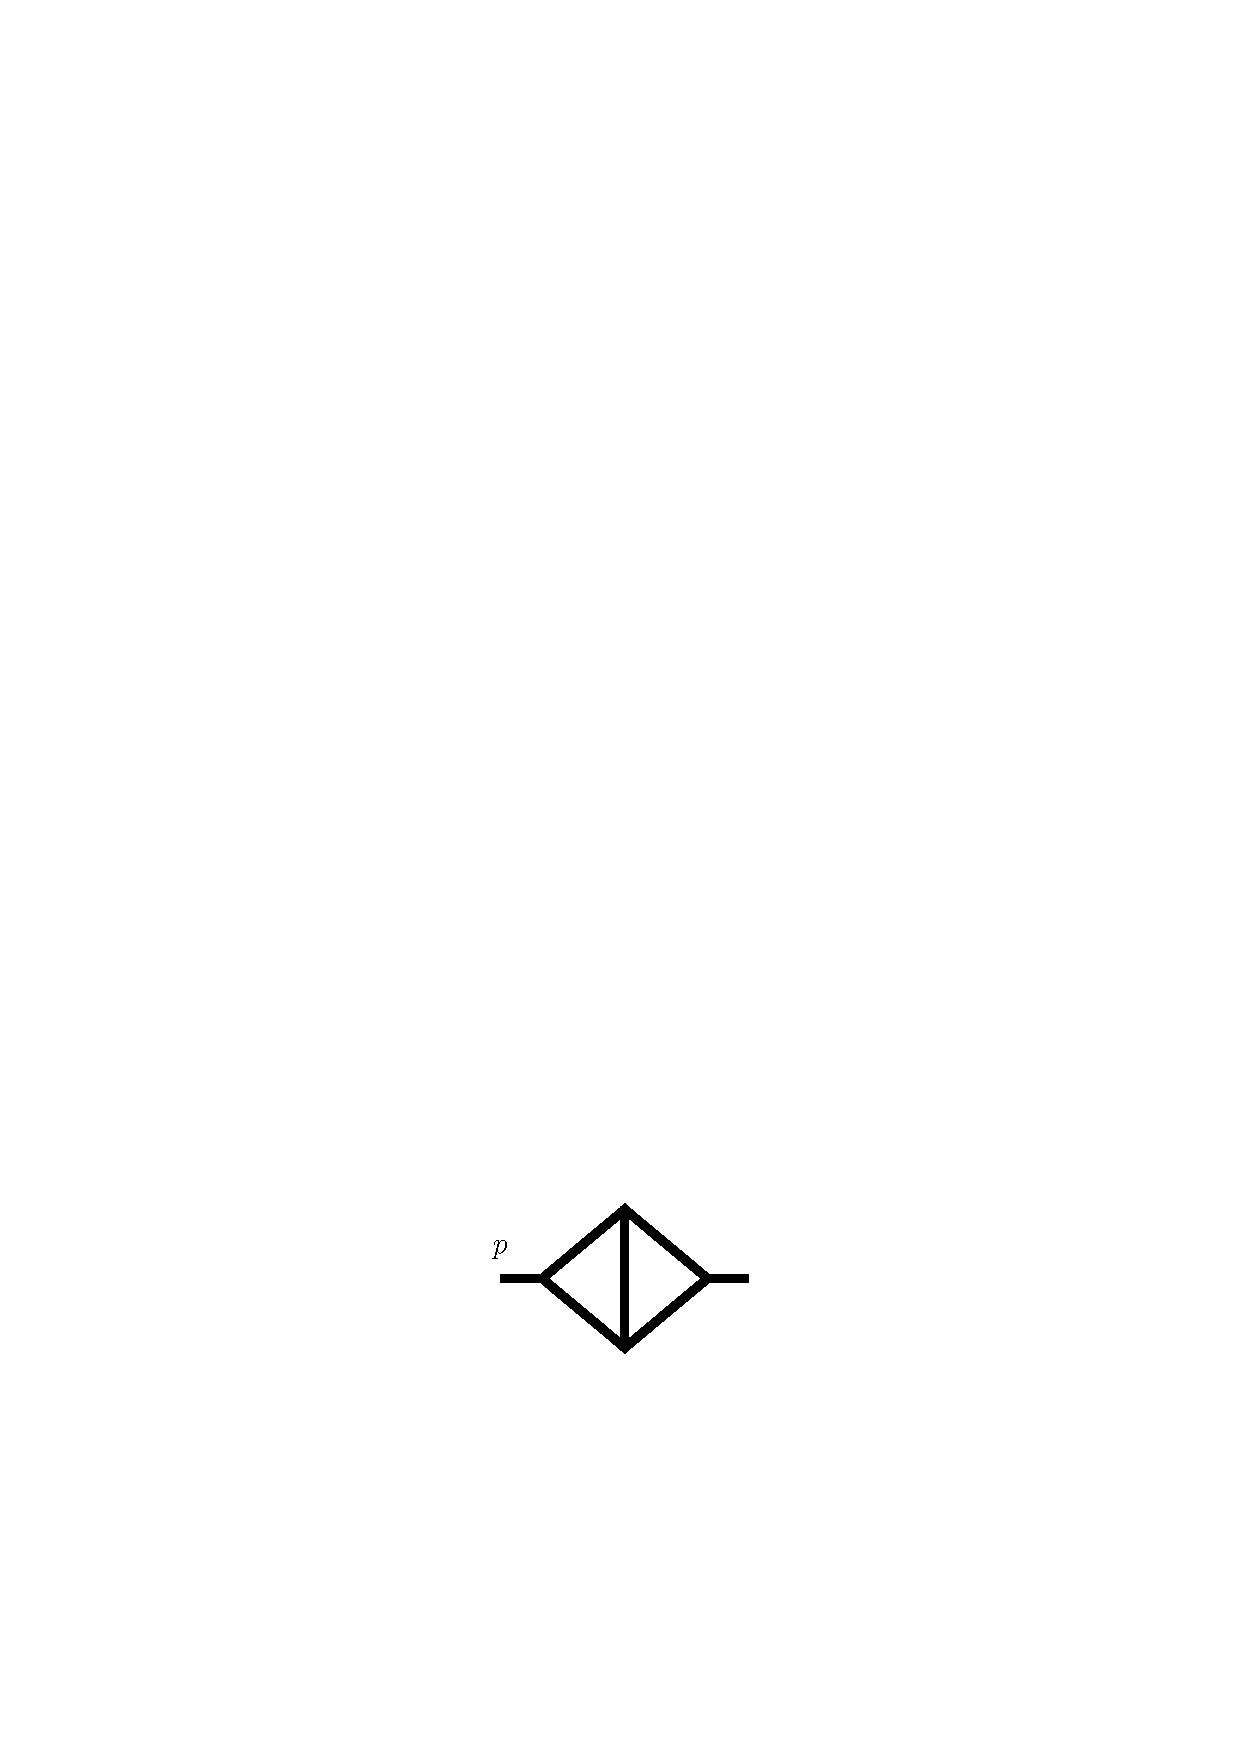
\includegraphics[width=3.cm]{ch4_loopints/figures/kite_integral.pdf}}}  \,.    
\end{equation}
All propagators are massless, and $s=p^2$.
Define the corresponding integral family. Write down the integration by parts identities for one of the triangle sub-integrals, and use them to express $F_{\text{kite}}\left(s; D\right)$ in terms of one-loop bubble integrals. Use the formula~\eqref{eq:Ibubblechapter4} to rewrite the latter in terms of $\Gamma$ functions, and show that
\begin{align} \label{eq:kite_result}
 F_{\text{kite}}\left(s; 4-2\eps \right) = \frac{6 \, \zeta_3}{-s} + \mathcal{O}\left(\eps\right) \,.
\end{align} 
For the solution see \hyperref[Sol:4.Kite]{chapter~5}.
\end{exer}


  \subsection{Obtaining the differential equations}
  \label{subsec:obtainingDE}
We know that for the bubble integral family~\eqref{deffamily} there are two master integrals, which can be chosen as in \eqn{choicemaster}.
We wish to know the derivatives of these integrals, as this would amount to knowing the derivative of any integral in the~family.

For any integral of the form~\eqref{deffamily}, it is straightforward to compute the derivative w.r.t.~$m^2$.
For example, we have
\begin{align}
\partial_{m^2} G_{a_1,a_2} = -a_1 G_{a_1 + 1,a_2} - a_2 G_{a_1, a_2 + 1 } \,.
\end{align}
Applying this for the two master integrals, we simply have
\begin{align}
\partial_{m^2} \begin{pmatrix}
G_{0,1}\\
G_{1,1} 
\end{pmatrix}
=
\begin{pmatrix}
-G_{2,0}\\
-2 \, G_{2,1} 
\end{pmatrix}\,.
\end{align}
Then, using the IBP relations~\eqref{IBPexamples}, we find
\begin{align}\label{DEexample1}
\partial_{m^2} \begin{pmatrix}
G_{0,1} \\
G_{1,1}
\end{pmatrix}
=
\left[
\begin{pmatrix}
0 & 0 \\
0 & \frac{-2}{4 m^2-s} 
\end{pmatrix}
+
\epsilon
\begin{pmatrix}
\frac{-1}{m^2} & 0 \\
\frac{-2}{m^2(4m^2-s)} & \frac{-4}{4 m^2-s} 
\end{pmatrix}
\right] \cdot
\begin{pmatrix}
G_{0,1} \\
G_{1,1}
\end{pmatrix}
\,.
\end{align}
Similarly, one can obtain the differential equations w.r.t.~$s$ by using $ \partial_s = 1/(2 s) p^{\mu} \partial_{p^{\mu}}$.
One finds
\begin{align}\label{DEexample1s}
\partial_{s} \begin{pmatrix}
G_{0,1} \\
G_{1,1}
\end{pmatrix}
=
\left[
\begin{pmatrix}
0 & 0 \\
0 & \frac{s-2 m^2}{s(4 m^2-s)} 
\end{pmatrix}
+
\epsilon
\begin{pmatrix}
0 & 0 \\
\frac{2}{s(4m^2-s)} & \frac{1}{4 m^2-s} \end{pmatrix}
\right] \cdot
\begin{pmatrix}
G_{0,1} \\
G_{1,1}
\end{pmatrix}
\,.
\end{align}

\subsection{Dimensional analysis and integrability check}
\label{sec:dimensionalanalysis}

There are two simple consistency checks we can perform of the differential equation matrices just obtained. 

\smallskip

{\it 1. Scaling relation}.
The integral $G_{a_1,a_2}(s,m^2;D)$ has overall (mass) dimension $D-2 a_1 - 2 a_2$. In other words, one can write
\begin{align}\label{eq:dimension}
G_{a_1,a_2}(s,m^2;D) = m^{D-2 a_1 -2 a_2} \, g(s/m^2;D)\,,
\end{align}
for some function $g$.
This implies the differential equation 
(dilatation relation)
\begin{align}
\left[ s \, \partial_s + m^2 \partial_{m^2} \right] G_{a_1,a_2} = (D/2-a_1-a_2) \, G_{a_1,a_2} \,.
\end{align}
Indeed, applying this differential operator to the massive bubble example, and using eqs.~\eqref{DEexample1} and~\eqref{DEexample1s}, we find
\begin{align}\label{eq:bubblerescaling}
 \left[ s \, \partial_s + m^2 \partial_{m^2} \right] 
 \begin{pmatrix}
G_{0,1} \\
G_{1,1}
\end{pmatrix} =
\begin{pmatrix}
-\eps & 0 \\
0 & -1-\eps 
\end{pmatrix} \cdot
\begin{pmatrix}
G_{0,1} \\
G_{1,1}
\end{pmatrix}\,.
\end{align}
Equation~\eqref{eq:bubblerescaling} is as expected. It is a diagonal matrix, with the diagonal entries corresponding to the scaling dimensions, measured in units of the dimension of $m^2$, cf.\ \eqn{eq:dimension}. The latter can be verified by dimensional analysis of the original definition in terms of loop integrals.

We remark that one could modify the definition of the master integrals, by simply rescaling them with a dimensional prefactor, to set their overall scaling dimension to zero. In our case $(m^2)^{\eps}$ and $(m^2)^{1+\eps}$ would achieve this. This would allow us to talk about single-variable differential equations in the variable $s/m^2$, as in \eqn{eq:dimension}.
However, in general we prefer not to include fractional terms such as $(m^2)^{\eps}$ in the definition, as this may obscure physical properties, e.g.\ when considering a limit $m\to 0$ or $m\to \infty$. Moreover, as we shall see, within the setup proposed here, dealing with multiple variables is not substantially more complicated as acompared to one variable.

\smallskip

{\it 2. Integrability conditions}.
A second check follows from the commutativity of partial derivatives, in our case $\partial_s \partial_{m^2}  -\partial_{m^2} \partial_{s} = 0$.
Applying this to our basis of master integrals, we get
\begin{align}\label{eq:integrability}
\left( \partial_{s} A_{m^2} - \partial_{m^2} A_{s} + A_{m^2} \cdot A_{s} - A_{s} \cdot A_{m^2} \right) \cdot \begin{pmatrix}
G_{0,1} \\
G_{1,1}
\end{pmatrix} =0 \,.
\end{align}  
One can verify indeed that the matrix appearing in \eqn{eq:integrability} vanishes identically.

\smallskip 

We close this subsection with a comment. Whenever one of the two checks discussed here fails, e.g.\ when one gets a non-vanishing matrix on the RHS of \eqn{eq:integrability}, this most likely points to some mistake in a calculation or implementation step. However, note that \eqn{eq:integrability} also admits solutions for non-vanishing matrices on the right-hand side if the master integrals are not linearly independent. It can indeed happen in practice that there are ``hidden'' IBP relations (that would e.g.\ be discovered by considering a larger set of IBP relations). In this case these checks may give hints for such missing relations. Note however that the converse is not true: successful scaling and integrability tests do not guarantee that one has found all IBP relations. 


\subsection{Canonical differential equations}
\label{sec:canonical}

The differential equations~\eqref{DEexample1} and~\eqref{DEexample1s} are already rather simple,
however by comparing to \eqn{eq:canonicalDEmanysingularpointsmultiplevariables} we see that they are not yet quite in canonical form.
In particular, they contain a $\eps^0$ term.
We will see in section~\ref{sec:dlog} how to directly find canonical differential equations but, for now,
let us proceed in a more pedestrian way.
We may attempt to ``integrate out'' the unwanted $\eps^0$ term, by changing basis from
\begin{align}
\vec{g} = 
 \begin{pmatrix}
G_{0,1}\\
G_{1,1}
\end{pmatrix}
\end{align}
to
\begin{align}
\vec{f} = T \cdot \vec{g}\,,
\end{align}
for some suitable invertible matrix $T$.
The differential equations for the new basis $\vec{f}$ are governed by \eqn{eq:defB}.
Demanding that this matrix is free of $\eps^0$ terms leads us to the following auxiliary problem:
\begin{align}
\partial_{m^2} T
=
- T  \cdot 
\begin{pmatrix}
0 & 0 \\
0 & \frac{-2}{4 m^2-s} 
\end{pmatrix}
\,,
\qquad 
\partial_{s} T
=
- T \cdot
\begin{pmatrix}
0 & 0 \\
0 & \frac{-2 m^2+s}{s(4 m^2-s)} 
\end{pmatrix}
 \,.
\end{align} 
This leads to the transformation matrix
\begin{align}
T = 
\begin{pmatrix}
1 & 0 \\
0 &\sqrt{(-s) (4m^2-s)}  
\end{pmatrix}
 \,,
\end{align}
and hence to the following new basis\footnote{In section~\ref{sec:dlog} we will see that this basis can be motivated in an entirely different way, without the need to analyse differential equations.}
\begin{align}\label{eq:UTbasisbubble}
\vec{f} = \begin{pmatrix}
G_{0,1}\\
\sqrt{(-s) (4m^2-s)} \, G_{1,1}
\end{pmatrix}\,.
\end{align}
Assuming $s<0,m^2>0$, one finds
\begin{align}\label{DEexample2}
\partial_{m^2} \, \vec{f} 
=
\epsilon \,
\begin{pmatrix}
\frac{-1}{m^2} & 0 \\
\frac{-2}{m^2 \sqrt{1-4 m^2/s}}  & \frac{-4 }{4 m^2-s}  
\end{pmatrix}
\cdot \vec{f} 
\,.
\end{align}
There is a similar equation for $\partial_s$.

So, structurally we have two differential equations 
\begin{align}
\partial_{m^2} \, \vec{f} = \eps\, A_{m^2} \cdot \vec{f} \,, \qquad
\partial_s \, \vec{f} = \eps\, A_{s} \cdot \vec{f} \,.
\end{align}
The two partial derivative equations can be combined in a single equation using the total differential $\d = \d s \, \partial_s + \d{m^2} \, \partial_{m^2}$.
Then we have
\begin{align}\label{canonical1}
\d \, \vec{f} =  \eps\,  (\d \tilde{A}) \cdot \vec{f} \,,
\end{align}
provided that $\tilde{A}$ satisfies
\begin{align}
\partial_{m^2} \, \tilde{A} = A_{m^2}  \,, \qquad
\partial_s \, \tilde{A} = A_{s}  \,.
\end{align}
We find the following $\tilde{A}$ solves these equations,
\begin{align}\label{canonical2}
\tilde{A} =   \begin{pmatrix}
-\log m^2 & 0 \\
-2 \log\left( \frac{\sqrt{1-4 m^2/s}-1}{ \sqrt{1-4 m^2/s} +1 } \right)  & - \log( 4 m^2-s )    
\end{pmatrix}  \,.
\end{align}
Equations~\eqref{canonical1} and~\eqref{canonical2} are an example of {\it canonical} differential equations for Feynman integrals~\cite{ch4Henn:2013pwa}.
The specific form~\eqref{canonical2} is an instance of the general case~\eqref{eq:canonicalDEmanysingularpointsmultiplevariables}, with $N=2$.
There are three alphabet letters, namely
\begin{align}\label{eq:alphabetbubble}
    \left\{ m^2, \frac{\sqrt{1-4 m^2/s}-1}{ \sqrt{1-4 m^2/s} +1 }, 4m^2-s \right\} \,.
\end{align}



\subsection{Solving the differential equations}
\label{subsec:solvingDE}

{\it General solution to the differential equations}.
Here we discuss how to solve the canonical differential equations.
We had already seen in section~\ref{sec:sepcialfunctionsfromDE} that the general solution takes the form of a path-ordered exponential, cf.~\eqref{eq:Wilsonlinesolution}. Adopting this equation to the present case, we have 
\begin{align}\label{eq:Wilsonlinesolutionbubble}
\vec{f}(\vec{x};\eps)  = {\mathbb P}\exp \left[\eps \int_{\cal C} \d \tilde{A}(\vec{x}') \right]  \cdot \vec{f}(\vec{x}_0;\eps) \,,
\end{align}
with $\tilde{A}$ from \eqn{canonical2}, and where $\vec{x}$ refers collectively to the set of kinematic variables $\vec{x}=(s,m^2)$, and $\vec{x}_0$ is an arbitrary base point for the integral, which takes the value $\vec{f}(\vec{x}_0;\eps)$ there. This corresponds to the fact that the system of first-order equations uniquely fixes the answer up to a boundary condition. We will discuss this presently.

There are simplifications thanks to the fact that the matrix in the exponent on the RHS of \eqn{eq:Wilsonlinesolutionbubble} is proportional to $\eps$. Therefore we can expand the exponential perturbatively in $\eps$. Moreover, due to the fact that the matrix on the RHS (cf.~\eqn{canonical2}) contains only logarithmic integration kernels, 
the answer are iterated integrals with the alphabet of \eqn{eq:alphabetbubble}.
In fact, we shall see presently that the answer up to the finite part is written in terms of much simpler functions. 
But this is not essential. The main message is that the class of special functions at our disposal is large enough to express the general solution to \eqn{canonical1} with \eqn{canonical2}.

\smallskip
In \eqn{eq:Wilsonlinesolutionbubble}, $\vec{f}(\vec{x}_0;\eps)$ is a boundary vector at a given base point $\vec{x}_{0}$.
As such, \eqn{eq:Wilsonlinesolutionbubble} expresses the general solution to the differential equations.
% 
In most cases, one is interested in the specific solution that corresponds to the Feynman integrals at hand.
This means that it is necessary to provide a boundary condition.
In other words, for a Feynman integral depending on multiple variables $\vec{x}$, one needs to know its value at one specific point $\vec{x}_{0}$.

\begin{important}{Fixing the boundary conditions from physical consistency conditions.}
One might naively think that a completely separate calculation is needed for this.
However, experience shows that one can obtain the boundary information from physical consistency conditions.
This approach is well known in the literature, but turns out to be especially easy within the canonical differential equations approach, 
which moreover offers additional insights~\cite{ch4Henn:2020lye}.
As a result, in most calculations this allows one to fix all integration constants, up to an overall normalisation.
\end{important}

The key is to consider the behaviour near singular points (or rather singular kinematic subvarieties) of the differential equations.
The singular points are  easily identified from the alphabet~\eqref{canonical2}. They correspond to kinematic configurations where alphabet letters tend to zero or infinity. In our case, this corresponds to $s=0, s=m^2, s=\infty, m^2=0, m^2 =\infty$.

In the present case, it turns out that $s=0$ is a suitable boundary configuration. The reason is that, physically, one knows that this limit is non-singular (due to the presence of the internal mass). In other words, we can simply set $p=0$ in \eqn{defbubble}. This reduces the bubble integral to a tadpole integral. 
However, since its normalisation factor in \eqn{eq:UTbasisbubble} vanishes, we do not even need to know its value. 
This fixes the boundary constant at $s=0$, up to the value of the tadpole integral. 
The calculation of the latter is elementary, with the result 
\begin{align}
G_{0,1}= \Gamma(\eps) \, \bigl(m^2\bigr)^{-\eps} \,,
\end{align}
which follows from \eqn{single_propagator} with $a=1$ and $D=2 -2 \eps$.
Therefore the boundary condition is
\begin{align}\label{boundarybubble1}
\vec{f}(s=0,m^2;D=2-2\eps) = 
 \begin{pmatrix}
\Gamma(\eps) (m^2)^{-\eps} \\
0
\end{pmatrix}\,.
\end{align}
This fixes the answer of the differential equation to all orders in $\eps$.



\smallskip

{\it Solution in terms of multiple polylogarithms}.
The alphabet \eqn{eq:alphabetbubble} can be rationalised using a simple change of variables.
Indeed, setting $s = -m^2 (1-x)^2/x$, and assuming $0<x<1$, \eqn{eq:alphabetbubble} becomes 
\begin{align}\label{eq:alphabetbubble2}
    \left\{ m^2, x , m^2 \frac{(1+x)^2}{x}  \right\} \,,
\end{align}
i.e.\ the alphabet, written in the independent variables $m^2$ and $x$ is simply
\begin{align}
    \left\{ m^2, x, 1+x \right\} \,.
\end{align}
This means that the answer can be written in terms of a special subclass of iterated integrals, called harmonic polylogarithms.\footnote{For more information on particular classes of special functions, and how to handle them efficiently, we refer interested readers to~\cite{ch4Duhr:2019wtr} and references therein.}
Moreover, the dependence on $m^2$ in the new alphabet becomes trivial, as it corresponds to the overall scale. We can therefore set $m^2=1$ without loss of generality, and solve the equations as a function of $x$ only. Equivalently, we could multiply all integrals by $(m^2)^{-\eps}$.

With this in mind, let us make the following final basis choice (the normalisation is motivated by \eqn{boundarybubble1}):
\begin{align}\label{eq:UTbasisbubblefinal}
\vec{f}(x;\eps) \coloneqq \frac{1}{(m^2)^{-\eps} \Gamma(\eps)}  \begin{pmatrix}
G_{0,1}\\
\sqrt{(-s) (4m^2-s)} \, G_{1,1}
\end{pmatrix}\,.
\end{align}
It satisfies the differential equations
\begin{align}\label{DEbubblefinalAtilde} 
\d \, \vec{f}(x;\eps) = \eps \, \d
 \begin{pmatrix}
0 & 0 \\
-2 \log x  & \log \frac{x}{(1+x)^2}  
\end{pmatrix} \cdot
 \vec{f}(x;\eps)\,,
\end{align}
with the boundary condition
\begin{align}\label{DEbubblefinalbdry}
\vec{f}(1;\eps)  =  \begin{pmatrix}
1\\
0
\end{pmatrix}\,.
\end{align}
More explicitly, \eqn{DEbubblefinalAtilde} is
\begin{align}\label{DEbubblefinalAtilde2} 
\partial_x \vec{f}(x;\eps) = \eps  \left[ \frac{1}{x} 
 \begin{pmatrix}
0 & 0 \\
-2   & 1   
\end{pmatrix} 
+
\frac{1}{1+x}
 \begin{pmatrix}
0 & 0 \\
0  & -2   
\end{pmatrix} 
\right] \cdot
 \vec{f}(x;\eps)\,.
\end{align}
We can now solve this equation, together with the boundary condition~\eqref{DEbubblefinalbdry}, order by order in $\eps$.
To do so, we set
\begin{align}
 \vec{f}(x;\eps) = \sum_{k \ge 0} \eps^k  \vec{f}^{(k)}(x) \,,
\end{align}
up to some order in $\eps$.
The key point is that the equations~\eqref{DEbubblefinalAtilde} decouple order by order in $\eps$,  when expressed in terms of $ \vec{f}^{(k)}(x)$.
For the first few orders, we straightforwardly find
\begin{align} 
\vec{f}^{(0)}(x) =  \begin{pmatrix}
1  \\
0     
\end{pmatrix} \,,
\end{align}
and 
\begin{align}\label{solbubbleweight1}
\vec{f}^{(1)}(x) =  \begin{pmatrix}
0  \\
-2 \log x     
\end{pmatrix} \,,
\end{align}
and 
\begin{align} \label{solbubbleweight2}
\vec{f}^{(2)}(x) =  \begin{pmatrix}
0  \\
4 \, {\rm Li}_{2}(-x) +4 \log x \log(1+x) -\log^2 x+\pi^2/3 
\end{pmatrix} \,.
\end{align} 
Recalling the definition~\eqref{eq:UTbasisbubblefinal},
this gives
\begin{align}
F_{2}\bigl(s,m^2;D=2- 2\eps\bigr) = 
\frac{\Gamma(1+\eps) (m^2)^{-\eps}}{\sqrt{(-s)(4 m^2-s)}} \left[   
- 2  \log\left( \frac{\sqrt{1-4 m^2/s}-1}{ \sqrt{1-4 m^2/s} +1 } \right) + {\cal O}(\eps) 
  \right] \,.
\end{align}
This agrees with \eqn{resbubbleexplicit}.
Furthermore, \eqn{solbubbleweight2} provides the next term in the $\eps$ expansion, and higher-order terms can be straightforwardly generated.

\newpage

\begin{exer}{The massive bubble integrals with the differential equations method}
\label{Ex:4.BubbleDE}
Write a \texttt{Mathematica} notebook for computing the massive bubble integrals~\eqref{deffamily} with $D=2-2\eps$ following step by step the discussion in section~\ref{sec:DEFeynmanintegrals}.
Use the package \textsc{LiteRed}~\cite{ch4Lee:2012cn} to perform the IBP reductions and differentiate the integrals. 
For the solution see the \texttt{Mathematica} notebook \href{https://scattering-amplitudes.mpp.mpg.de/scattering-amplitudes-in-qft/Exercises/}{\tt Ex4.12\_BubbleDE.wl}~\cite{ch4website-ch4}.

\end{exer}





 
\section{Feynman integrals of uniform transcendental weight}
\label{sec:dlog}

In the previous subsections, we have discussed special functions appearing in Feynman diagrams.
We have seen in the preceding chapters that they satisfy simple, canonical differential equations. 
However, we have also seen that the equations have a gauge degree of freedom, which corresponds to making a basis choice for the coupled system of $N$ equations. This freedom implies that the DE may be written in an equivalent, albeit unnecessarily complicated form. Therefore an important question is: how can we make sure that the equations we get for Feynman integrals will have the desired simple, canonical form?

We address this problem in this section. This builds on the observations of section~\ref{subsec:comments} that pure uniform weight functions satisfy canonical differential equations. In this section we present a conjecture that gives a criterium for when a Feynman integral evaluates to such functions. Taken together, this provides the information for how to choose a set of Feynman integrals that satisfy canonical differential equations.   


\subsection{Connection to differential equations and (unitarity) cuts}
\label{sec:DEandCuts}

We have already seen in section~\ref{subsec:comments} that, in the context of the differential equations satisfied by Feynman integrals, it is natural to consider discontinuities.
It turns out that there is a useful connection to (generalised) unitarity methods.

This is based on the important observation that unitarity cuts of an integral satisfy the same differential
equations, albeit with different boundary conditions.
We can see this in the following way~\cite{ch4Anastasiou:2002yz}.
When we ``cut'' a propagator, we effectively replace $1/(-k^2+m^2)$ by $\delta(-k^2+m^2)$.
As was discussed in section~\ref{sec:3.3} of chapter~\ref{ch:loopamps},
the cut can be written as a difference of propagators with different $\i 0$ prescriptions.
However, this prescription does not affect the derivation of the IBP relations, and hence one gets the same differential equations.
Of course, the boundary values of the cut integrals differ from the original ones, and in particular one could put to zero integrals that obviously vanish on a cut because the relevant cut propagators are absent.

Consider the one-loop massive bubble integrals $G_{1,1}$ and $G_{1,0}$ of \eqn{defbubble} as an example.
Applying an $s$-channel unitarity cut, and setting\footnote{One key feature of the canonical differential equations is that their RHS vanishes for $\eps=0$.
It is therefore interesting to ask whether we can solve for the $\eps=0$ part of the differential equations. However, it is also interesting (albeit more involved) to study cut integrals for general $D$.} $D=2$ we obtain
\begin{align}\label{eq:B11cutintegral}
G_{1,1} \longrightarrow \int  \d^{2}k \, \delta\bigl(-k^2+m^2 \bigr) \, \delta\bigl(- (k+p)^2+m^2 \bigr)  = \frac{1}{\sqrt{(-s)(4 m^2-s)}} \,.
\end{align}
This is exactly the factor we introduced in \eqn{eq:UTbasisbubble} to remove the $\eps=0$ part of the differential equation.
Performing the same cut on the tadpole integral $G_{1,0}$ vanishes, simply because it is
missing one propagator that was cut. 
Indeed, by cutting all propagators---whose number happens to coincide here with the space-time dimension $D=2$---we are taking a so-called \emph{maximal cut}. This allows us to focus on a given integral sector.
In terms of the differential equations, this means that this cut describes a block of the differential equations,
whose size corresponds to the number of relevant master integrals.
In the present case, there is just one master integral with two propagators, so the block corresponds of one element
of the differential equations.

We can also learn something about the tadpole integral, by considering generalised unitarity cuts. 
The most obvious is to cut the one propagator that is present. It is instructive to do this:
\begin{align}\label{eq:B10cutintegral}
G_{1,0} \longrightarrow \int  \d^{2}k \, \delta\bigl(-k^2+m^2\bigr)   \,.
\end{align}
It is convenient to introduce two light-like vectors $p_1$ and $p_2$, with $p_1^2 = p_2^2 = 0$, such that $p=p_1 + p_2$, and $2 \, p_1 \cdot p_2 = s$.
This allows us to parametrise $k= \beta_1 p_1 + \beta_2 p_2$. 
Taking into account the Jacobian from the change of variables, and using the delta function to fix one integration, we find
\begin{align}
G_{1,0} \longrightarrow \int \d\beta_1 \d\beta_2 \, s \, \delta\bigl(-s \beta_1 \beta_2 + m^2\bigr) = \int \frac{\d\beta_2}{\beta_2} \,.
\end{align}
Unlike \eqn{eq:B11cutintegral}, here the integrations are not fully fixed.
Moreover, the first integration has produced a new singularity, $1/\beta_2$, that was not present initially.
This is a typical situation in generalised unitarity. 
We can define a further cut and localise the integral at one of its singularities, either $\beta_2= 0$ or $\beta_2 = \infty$.
The result is just $\pm 1$, which confirms the normalisation choice in \eqn{eq:UTbasisbubble}.


\subsection{Integrals with constant leading singularities and uniform weight conjecture}

The calculations above provided useful insight about diagonal blocks of the differential equations (in the present case, the diagonal elements, since the block size happened to be one). Can one also learn something about the off-diagonal terms with this method?
The answer---conjecturally---is yes. The idea is first to think of the above calculations not of changing the integrand, but instead of changing the integration contour.
The original integration is over two-dimensional Minkowski space. In the calculations above, we have effectively replaced this by certain residue calculations.
The idea then is to generalise this to arbitrary residues we can take for a given loop integrand.
In the case where those residues completely localise the loop integrations, one speaks specifically of \emph{leading singularities}. 
We know that leading singularities that correspond to maximal cuts inform us about diagonal blocks of the differential equations. 
The assumption is that the other residues ``know about'' the off-diagonal parts, even though we do not know the precise mapping.
However, for the present purposes, this precise map is not relevant: if we can normalise all leading singularities 
to constants, then their derivatives will obviously be trivial. 
This gives us a useful tool for obtaining differential equations whose RHS is proportional to $\eps$.

How does one see that all leading singularities are kinematic-independent constants?
Let us review the tadpole and bubble integrands from this viewpoint.
As explained, we now focus on the {\it integrand},
\begin{align}
    \omega_{1,0} = \frac{\d^2k}{-k^2+m^2} \propto \frac{\d\beta_1 \d\beta_2 \, s}{-s \beta_1 \beta_2 + m^2} \,,
\end{align}
where we have used the same loop parametrisation as above.
Integrating one variable at a time, we can write this in the following way,
\begin{align}
\omega_{1,0} \propto \d \log \bigl(-s \beta_1 \beta_2 + m^2 \bigr) \, \d\log \bigl(\beta_2 \bigr) \,.
\end{align}
Here $\d= \d\beta_1 \, \partial_{\beta_1} + \d\beta_2 \, \partial_{\beta_2}$. The differential forms satisfy $\d\beta_i \d\beta_j = - \d\beta_j \d\beta_i$, 
and hence e.g.~$\d\beta_2 \d\beta_2 =0$.
In other words, upon further changing variables, the form~reads
\begin{align} \label{eq:omega10dlog}
\omega_{1,0} \propto \frac{\d\tau_1}{\tau_1} \frac{\d\tau_2}{\tau_2} \,.
\end{align}
This makes it clear that any leading singularity of this integral evaluates to a constant, and hence that any of its derivatives vanishes, as desired.

Repeating this analysis for the bubble is slightly more interesting. We leave it as an exercise to readers.
The result can be written as
\begin{align} \label{eq:bubble_dlog} \begin{aligned}
    \omega_{1,1} = \ & \frac{\d^2k}{(-k^2+m^2)[-(k+p)^2+m^2]}\,, \\
     \propto &  \frac{1}{\sqrt{(-s)(4m^2-s)}} \, \d\log\left[\frac{-k^2+m^2}{(k-k_{\pm})^2} \right] \, \d\log\left[\frac{-(k+p)^2+m^2}{(k-k_{\pm})^2} \right] \,.
\end{aligned} \end{align}
Here $k_{\pm}$ is any of the two solutions to the cut equations $-k^2+m^2=-(k+p)^2+m^2=0$.
This expression makes it manifest that $\omega_{1,1}$ has only logarithmic singularities (i.e., of type $\d x/x$), and its maximal residue (i.e., its leading singularity) is 
\begin{align}\label{massiveleadingsing}
    \oint \omega_{1,1} \propto \frac{1}{\sqrt{(-s)(4m^2-s)}} \,.
\end{align}
Therefore we conclude that the integral $ {\sqrt{(-s)(4m^2-s)}} \, \int  \omega_{1,1}$ is a good basis integral that may lead to canonical differential equations. 
Indeed, note that this is consistent with \eqn{resbubbleexplicit}.


\begin{exer}{``$\d \log$'' form of the massive bubble integrand with $D=2$}
\label{Ex:4.BubbleCut}
Use the parameterisation introduced above ($k=\beta_1 p_1 + \beta_2 p_2$) to prove that the integrand of the massive bubble in $D=2$ dimensions can be expressed as a ``$\d \log$'' form. Show that the latter is equivalent to the momentum-space $\d \log$ form in \eqn{eq:bubble_dlog}. 
For the solution see \hyperref[Sol:4.BubbleCut]{chapter~5}.
\end{exer}


Interestingly, the question of which Feynman integrals evaluate to uniform weight functions was previously studied 
independently from the differential equations.
Understanding initially came from studies of scattering amplitudes in ${\mathcal N} =4$ super Yang-Mills theory, 
but it turned out that the observations made there were applicable more generally~\cite{ch4Arkani-Hamed:2010pyv,ch4Henn:2013pwa}. 
This led to the following conjecture. A Feynman integral integrates to a pure function if 
\begin{enumerate}
\item its integrand, and iterated residues thereof, only contains simple poles,
\item the maximal residues are normalised to constants.
\end{enumerate}
These two criteria are in one-to-one correspondence to the properties discussed above. 
The first requirement is intended to remove less than maximal weight functions, and therefore lead to integrals with uniform and maximal weight. 
See exercise~\ref{Ex:4.KiteLS} for an example of an integrand with a double pole, which is a sign for a weight-drop. 
As computed explicitly in exercise~\ref{Ex:4.Kite}), the answer has weight three, which is less than the maximal weight four expected for two-loop integrals in four dimensions.
The second requirement addresses another potential problem: if an integral is a sum of maximal weight functions with different algebraic prefactors, 
this spoils the desired simple structure under differentiation. Normalising all prefactors to kinematic-independent constants solves this issue.


\begin{important}{Integrand conjecture as a practical tool for finding canonical differential equations.}
The above integrand conjecture has proven preciously useful for choosing bases of Feynman integrals that satisfy canonical differential equations. What renders this method particularly powerful is that it can be used at the level of the loop integrand, independently of questions about IBP identities, and without knowledge of the differential equations.
\end{important}


\vspace{-0.6cm}
\begin{exer}{An integrand with double poles: the two-loop kite in $D=4$}
\label{Ex:4.KiteLS}
Compute the four-dimensional maximal cut of the two-loop kite integral defined in exercise~\ref{Ex:4.Kite}, and show that---on the maximal cut---its integrand has a double pole. Hint: introduce two auxiliary light-like momenta $p_1$ and $p_2$ ($p_i^2=0$) such that $p=p_1+p_2$, and use the spinors associated with them to construct a basis in which to expand the loop momenta.
For the solution see \hyperref[Sol:4.KiteLS]{chapter~5}.
\end{exer}


\vspace{-0.6cm}
\begin{exer}{Computing leading singularities with \textsc{DlogBasis}}
\label{Ex:4.dlogs}
%
The \texttt{Mathematica} package \textsc{DlogBasis}~\cite{ch4Henn:2020lye} provides a suite of tools for computing leading singularities and checking whether a given integrand can be cast into $\d \log$ form, based on the partial fractioning procedure we used to solve exercise~\ref{Ex:4.BubbleCut}. Use \textsc{DlogBasis} to do the following.
\begin{enumerate}[a)]
\item Verify the leading singularities of the massive tadpole and bubble integrals given in eqs.~\eqref{eq:omega10dlog} and~\eqref{massiveleadingsing}.
\item Verify that the integrand of the two-loop kite integral with $D=4$ studied in exercise~\ref{Ex:4.KiteLS} has a double pole.
\item Consider the integrands of the following massless box and triangle integrals,
\vspace{-0.2cm}
\begin{align}
 \int \omega^{\text{box}} = \vcenter{\hbox{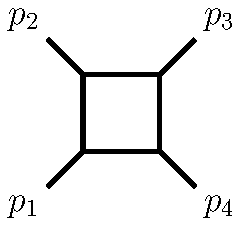
\includegraphics[width=1.8cm]{ch4_loopints/figures/box_small.pdf}}} \,,  \ \
 \int \omega^{\text{tr.}}_{s} = \vcenter{\hbox{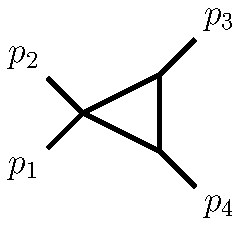
\includegraphics[width=1.8cm]{ch4_loopints/figures/triangle_s_small.pdf}}} \,, \ \
 \int \omega^{\text{tr.}}_{t} = \vcenter{\hbox{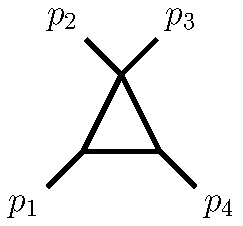
\includegraphics[width=1.8cm]{ch4_loopints/figures/triangle_t_small.pdf}}} \,, 
\end{align}
\vspace{-0.1cm}
with $p_i^2 = 0$.
Show that their leading singularities in $D=4$ dimensions are
\begin{align}
\oint \omega^{\text{box}} \propto \frac{1}{s \, t} \,, \qquad \quad \oint \omega^{\text{tr.}}_s \propto \frac{1}{s} \,,  \qquad \quad
  \oint \omega^{\text{tr.}}_t \propto \frac{1}{t} \,,
\end{align}
where $s=2 \, p_1 \cdot p_2$ and $t = 2\, p_2 \cdot p_3$. Parametrise the integrands using \textsc{DlogBasis}' utilities to expand the loop momentum in a four-dimensional basis constructed from the spinors associated with $p_1$ and $p_2$.
\end{enumerate}
%
For the solution see the \texttt{Mathematica} notebook \break \href{https://scattering-amplitudes.mpp.mpg.de/scattering-amplitudes-in-qft/Exercises/}{\texttt{Ex4.15\_LeadingSingularities.wl}}~\cite{ch4website-ch4}. 

\end{exer}


\begin{exer}{The box integrals with the differential equations method}
\label{Ex:4.BoxDE}
%
Write a \texttt{Mathematica} notebook to compute the massless one-loop box integrals,
\begin{align} \label{eq:box_def}
G^{\mathrm{box}}_{a_1,a_2,a_3,a_4} = \int \frac{\d^D k}{\i \pi^{D/2}} \frac{1}{D_1^{a_1} D_2^{a_2} D_3^{a_3} D_4^{a_4} }\,,
\end{align}
where
\begin{align}\begin{alignedat}{2}
& D_1 =  -k^2 - \i 0\,,  & \quad & D_3 =  -(k+p_1+p_2)^2 - \i 0 \,, \\
& D_2 = -(k+p_1)^2 - \i 0 \,, & \qquad \quad & D_4 = - (k-p_4)^2 - \i 0\,,
\end{alignedat}\end{align}
with $p_i^2=0$ and $p_1+p_2+p_3+p_4=0$, using the method of DEs.
Parameterise the kinematics in terms of $s = 2 \, p_1 \cdot p_2$ and $t = 2 \, p_2 \cdot p_3$, and assume that $s<0$ and $t<0$. In this domain, called Euclidean region, the integrals are real valued, and we may thus neglect the $\i 0$'s.
Use the package \textsc{LiteRed}~\cite{ch4Lee:2012cn} to perform the IBP reductions and differentiate the integrals. 
\begin{enumerate}[a)]
\item Define the family and solve the IBP relations to find a basis of master integrals. 
\item Compute the DEs satisfied by the master integrals as functions of $s$ and $t$. Check the scaling relation and the integrability conditions.
\item Change basis of master integrals to
\begin{align} \label{eq:fdef}
\vec{f}(s,t;\eps) = c(\eps) \, \begin{pmatrix}  
   s \, t \, G^{\text{box}}_{1,1,1,1} \\
   s \, G^{\text{box}}_{1,1,1,0} \\ 
   t \, G^{\text{box}}_{1,1,0,1}
\end{pmatrix} \,,
\end{align}
where $c(\eps) = \eps^2 \, \text{e}^{\eps \gamma_{\text{E}}}$. From exercise~\ref{Ex:4.dlogs} we know that, for $D=4$, the integrals in $\vec{f}$ contain only simple poles at the integrand level, and have constant leading singularities.
Compute the transformation matrix and the DEs satisfied by $\vec{f}$. Verify that the latter are in canonical form.

\item Change variables from $(s,t)$ to $(s,x)$, with $x=t/s$.

\item Determine the weight-0 boundary values. Use the results of exercise~\ref{Ex:MasslessBubble} for the master integrals of bubble type. Fix the remaining value by imposing that the solution to the DEs is finite at $u=-s-t = 0$ ($x=-1$). Write a function which produces the symbol of the solution up to a given order in $\eps$.

\item Determine the boundary values at the basepoint $x_0 = 1$ order by order in $\eps$. 
Write a function which produces the analytic solution up to a given order in $\eps$.

\item Verify that the solution for the box integral $G^{\text{box}}_{1,1,1,1}$ agrees with the result obtained through the Mellin-Barnes method in \eqn{eq:F4final}.

\end{enumerate}
For the solution see \hyperref[Sol:4.BoxDE]{chapter~5} and the \texttt{Mathematica} notebook \href{https://scattering-amplitudes.mpp.mpg.de/scattering-amplitudes-in-qft/Exercises/}{\texttt{Ex4.16\_BoxDE.wl}}~\cite{ch4website-ch4}. 

\end{exer}



\begin{thebibliography}{99.}
%\cite{Peskin:1995ev}
\bibitem{ch4Peskin:1995ev}
M.~E.~Peskin and D.~V.~Schroeder,
``An Introduction to quantum field theory,''
Addison-Wesley, 1995,
ISBN 978-0-201-50397-5.

%\cite{Smirnov:2012gma}
\bibitem{ch4Smirnov:2012gma}
V.~A.~Smirnov,
``Analytic tools for Feynman integrals,''
Springer Tracts Mod. Phys. \textbf{250} (2012), 1-296
doi:10.1007/978-3-642-34886-0.

%\cite{Weinzierl:2022eaz}
\bibitem{ch4Weinzierl:2022eaz}
S.~Weinzierl,
``Feynman Integrals,''
doi:10.1007/978-3-030-99558-4
[arXiv:2201.03593 [hep-th]].

%\cite{Henn:2014qga}
\bibitem{ch4Henn:2014qga}
J.~M.~Henn,
``Lectures on differential equations for Feynman integrals,''
J. Phys. A \textbf{48} (2015), 153001
doi:10.1088/1751-8113/48/15/153001
[arXiv:1412.2296 [hep-ph]].

%\cite{Lee:2012cn}
\bibitem{ch4Lee:2012cn}
R.~N.~Lee,
``Presenting LiteRed: a tool for the Loop InTEgrals REDuction,''
[arXiv:1212.2685 [hep-ph]].

%\cite{Agarwal:2021ais}
\bibitem{ch4Agarwal:2021ais}
N.~Agarwal, L.~Magnea, C.~Signorile-Signorile and A.~Tripathi,
``The infrared structure of perturbative gauge theories,''
Phys. Rept. \textbf{994} (2023), 1-120
doi:10.1016/j.physrep.2022.10.001
[arXiv:2112.07099 [hep-ph]].

%\cite{Panzer:2014caa}
\bibitem{ch4Panzer:2014caa}
E.~Panzer,
``Algorithms for the symbolic integration of hyperlogarithms with applications to Feynman integrals,''
Comput. Phys. Commun. \textbf{188} (2015), 148-166
doi:10.1016/j.cpc.2014.10.019
[arXiv:1403.3385 [hep-th]].

%\cite{Czakon:2005rk}
\bibitem{ch4Czakon:2005rk}
M.~Czakon,
``Automatized analytic continuation of Mellin-Barnes integrals,''
Comput. Phys. Commun. \textbf{175} (2006), 559-571
doi:10.1016/j.cpc.2006.07.002
[arXiv:hep-ph/0511200 [hep-ph]].

%\cite{Kotikov:2002ab}
\bibitem{ch4Kotikov:2002ab}
A.~V.~Kotikov and L.~N.~Lipatov,
``DGLAP and BFKL equations in the $N=4$ supersymmetric gauge theory,''
Nucl. Phys. B \textbf{661} (2003), 19-61
[erratum: Nucl. Phys. B \textbf{685} (2004), 405-407]
doi:10.1016/S0550-3213(03)00264-5
[arXiv:hep-ph/0208220 [hep-ph]].

%\cite{Zagier:2007knq}
\bibitem{ch4Zagier:2007knq}
D.~Zagier,
``The Dilogarithm Function,''
doi:10.1007/978-3-540-30308-4\_1.

%\cite{Henn:2013pwa}
\bibitem{ch4Henn:2013pwa}
J.~M.~Henn,
``Multiloop integrals in dimensional regularization made simple,''
Phys. Rev. Lett. \textbf{110} (2013), 251601
doi:10.1103/PhysRevLett.110.251601
[arXiv:1304.1806 [hep-th]].

%\cite{Henn:2020lye}
\bibitem{ch4Henn:2020lye}
J.~Henn, B.~Mistlberger, V.~A.~Smirnov and P.~Wasser,
``Constructing d-log integrands and computing master integrals for three-loop four-particle scattering,''
JHEP \textbf{04} (2020), 167
doi:10.1007/JHEP04(2020)167
[arXiv:2002.09492 [hep-ph]].

%\cite{Muller-Stach:2012tgj}
\bibitem{ch4Muller-Stach:2012tgj}
S.~M\"uller-Stach, S.~Weinzierl and R.~Zayadeh,
``Picard-Fuchs equations for Feynman integrals,''
Commun. Math. Phys. \textbf{326} (2014), 237-249
doi:10.1007/s00220-013-1838-3
[arXiv:1212.4389 [hep-ph]].

%\cite{Henn:2020omi}
\bibitem{ch4Henn:2020omi}
J.~M.~Henn,
``What Can We Learn About QCD and Collider Physics from N=4 Super Yang\textendash{}Mills?,''
Ann. Rev. Nucl. Part. Sci. \textbf{71} (2021), 87-112
doi:10.1146/annurev-nucl-102819-100428
[arXiv:2006.00361 [hep-th]].

%\cite{Goncharov:2010jf}
\bibitem{ch4Goncharov:2010jf}
A.~B.~Goncharov, M.~Spradlin, C.~Vergu and A.~Volovich,
``Classical Polylogarithms for Amplitudes and Wilson Loops,''
Phys. Rev. Lett. \textbf{105} (2010), 151605
doi:10.1103/PhysRevLett.105.151605
[arXiv:1006.5703 [hep-th]].

%\cite{Duhr:2012fh}
\bibitem{ch4Duhr:2012fh}
C.~Duhr,
``Hopf algebras, coproducts and symbols: an application to Higgs boson amplitudes,''
JHEP \textbf{08} (2012), 043
doi:10.1007/JHEP08(2012)043
[arXiv:1203.0454 [hep-ph]].

%\cite{Lee:2014ioa}
\bibitem{ch4Lee:2014ioa}
R.~N.~Lee,
``Reducing differential equations for multiloop master integrals,''
JHEP \textbf{04} (2015), 108
doi:10.1007/JHEP04(2015)108
[arXiv:1411.0911 [hep-ph]].

%\cite{Duhr:2019wtr}
\bibitem{ch4Duhr:2019wtr}
C.~Duhr,
``Function Theory for Multiloop Feynman Integrals,''
Ann. Rev. Nucl. Part. Sci. \textbf{69} (2019), 15-39
doi:10.1146/annurev-nucl-101918-023551.

%\cite{Bourjaily:2022bwx}
\bibitem{ch4Bourjaily:2022bwx}
J.~L.~Bourjaily, J.~Broedel, E.~Chaubey, C.~Duhr, H.~Frellesvig, M.~Hidding, R.~Marzucca, A.~J.~McLeod, M.~Spradlin and L.~Tancredi, \textit{et al.}
``Functions Beyond Multiple Polylogarithms for Precision Collider Physics,''
[arXiv:2203.07088 [hep-ph]].

%\cite{Laporta:2000dsw}
\bibitem{ch4Laporta:2000dsw}
S.~Laporta,
``High precision calculation of multiloop Feynman integrals by difference equations,''
Int. J. Mod. Phys. A \textbf{15} (2000), 5087-5159
doi:10.1142/S0217751X00002159
[arXiv:hep-ph/0102033 [hep-ph]].

%\cite{Lee:2013hzt}
\bibitem{ch4Lee:2013hzt}
R.~N.~Lee and A.~A.~Pomeransky,
``Critical points and number of master integrals,''
JHEP \textbf{11} (2013), 165
doi:10.1007/JHEP11(2013)165
[arXiv:1308.6676 [hep-ph]].

%\cite{Bitoun:2017nre}
\bibitem{ch4Bitoun:2017nre}
T.~Bitoun, C.~Bogner, R.~P.~Klausen and E.~Panzer,
``Feynman integral relations from parametric annihilators,''
Lett. Math. Phys. \textbf{109} (2019) no.3, 497-564
doi:10.1007/s11005-018-1114-8
[arXiv:1712.09215 [hep-th]].

%\cite{Anastasiou:2002yz}
\bibitem{ch4Anastasiou:2002yz}
C.~Anastasiou and K.~Melnikov,
``Higgs boson production at hadron colliders in NNLO QCD,''
Nucl. Phys. B \textbf{646} (2002), 220-256
doi:10.1016/S0550-3213(02)00837-4
[arXiv:hep-ph/0207004 [hep-ph]].

%\cite{Arkani-Hamed:2010pyv}
\bibitem{ch4Arkani-Hamed:2010pyv}
N.~Arkani-Hamed, J.~L.~Bourjaily, F.~Cachazo and J.~Trnka,
``Local Integrals for Planar Scattering Amplitudes,''
JHEP \textbf{06} (2012), 125
doi:10.1007/JHEP06(2012)125
[arXiv:1012.6032 [hep-th]].

%\cite{Chicherin:2021dyp}
\bibitem{ch4Chicherin:2021dyp}
D.~Chicherin, V.~Sotnikov and S.~Zoia,
``Pentagon functions for one-mass planar scattering amplitudes,''
JHEP \textbf{01} (2022), 096
doi:10.1007/JHEP01(2022)096
[arXiv:2110.10111 [hep-ph]].

\bibitem{ch4website-ch4}
\href{https://scattering-amplitudes.mpp.mpg.de/scattering-amplitudes-in-qft/Exercises/}{https://scattering-amplitudes.mpp.mpg.de/scattering-amplitudes-in-qft/Exercises/}.
\end{thebibliography}
